\chapter{Algoritmi proposti}

Gli algoritmi presentati in questo documento, pur basandosi su approcci 
concettualmente diversi, possono essere classificati in due categorie 
principali sulla base delle proprietà che esaminano del politopo di partenza: 
\textit{algoritmi con analisi dei verticio} e 
\textit{algoritmi con analisi degli iperpiani}.\\

In entrambi i casi i meccanismi implementati dagli algoritmi in esame
si basano su computazioni geometriche come il calcolo di aree, traslazioni, calcolo di intersezioni
inversioni di iperpiani e la costruzione di gusci convessi. 
Tali tecniche consentono di ridurre la complessità degli oggetti geometrici, mantenendo una 
buona approssimazione delle loro caratteristiche originali. A supporto di questi calcoli, 
vengono impiegati algoritmi classici della geometria computazionale come l'algoritmo di 
\textit{Jarvis March} (conosciuto anche come \textit{Gift Wrapping})
\cite{JarvisMarchAlgorithm}, utilizzato per il calcolo di gusci convessi 
in diversi spazi dimensionali.\\

Le rappresentazioni visive fornite di seguito, create con software AutoCad,
illustrano il funzionamento degli algoritmi, evidenziando passo per passo i 
processi geometrici e decisionali alla base della loro esecuzione. 
Vengono inoltre riportati esempi rappresentativi delle loro applicazioni, 
che mostrano come gli algoritmi gestiscono i casi reali.

\pagebreak
\section{Approssimazioni tramite analisi delle proprietà dei vertici}
Gli algoritmi presentati in questo capitolo, pur essendo fondati su principi operativi 
differenti, condividono l'approccio di analizzare i vertici del guscio convesso iniziale 
secondo diversi criteri geometrici e strutturali.

\subsection{Ipotesi di Algoritmo Cutting Smaller Angle (CSA)}

L'algoritmo CSA si basa sull'eliminazione dei vertici che formano un angolo interno al 
politopo inferiore rispetto agli altri. Questa strategia si fonda sull'assunzione che 
gli angoli più acuti siano associati a vertici che possono essere considerati outlier 
rispetto alla geometria complessiva del politopo originale. 
Tali vertici potrebbero infatti distorcere l'accuratezza della rappresentazione approssimata.

\begin{center}
    Esempi di approssimazione:
\end{center}
\begin{figure}[H]
    \centering
    \begin{tabular}{ccc}
        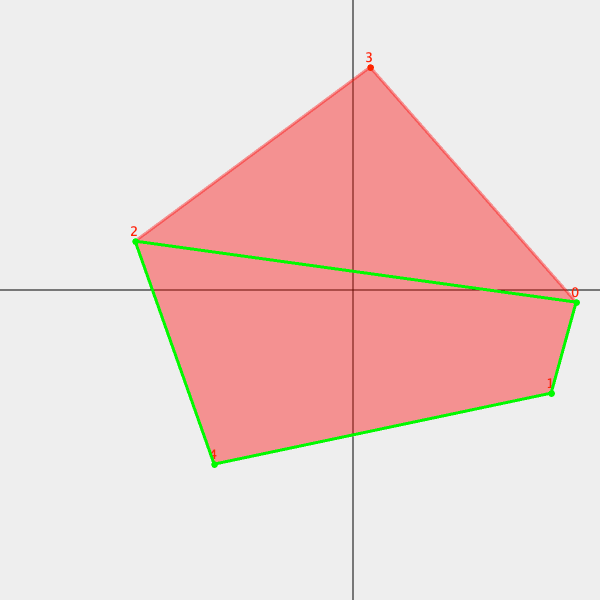
\includegraphics[width=0.3\textwidth]{media/CuttingSmallerAngle/5_4.png} &
        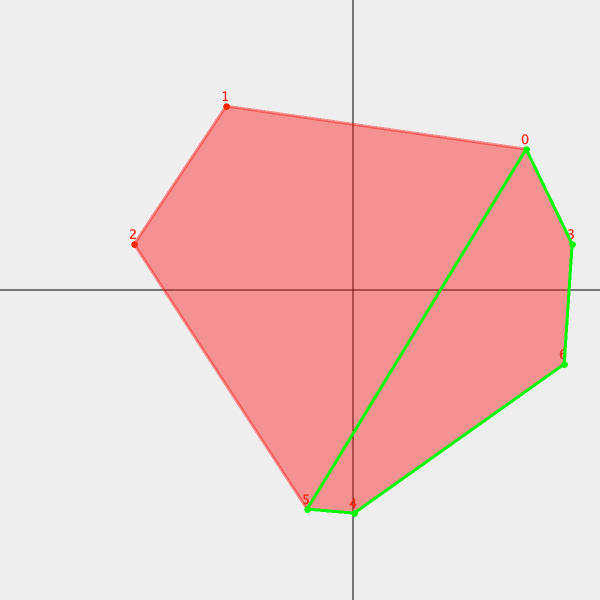
\includegraphics[width=0.3\textwidth]{media/CuttingSmallerAngle/7_5.png} &
        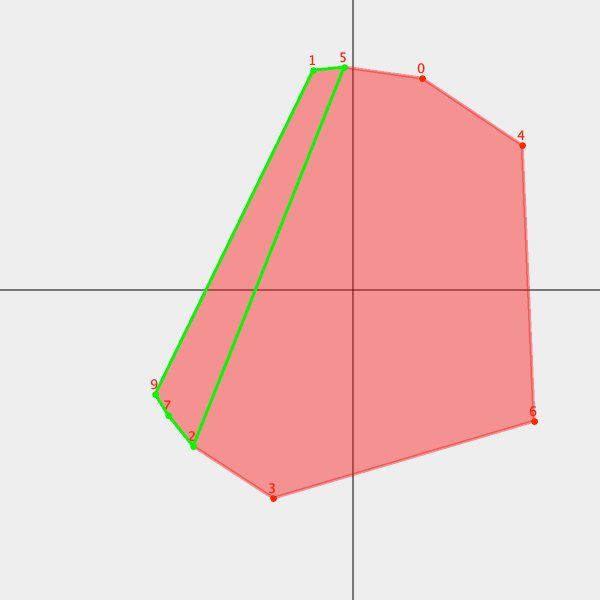
\includegraphics[width=0.3\textwidth]{media/CuttingSmallerAngle/9_5.png} \\
        (a) E = 5, h = 4 & (b) E = 7, h = 5 & (c) E = 9, h = 5
    \end{tabular}
\end{figure}

Le approssimazioni ottenute da questo algoritmo portano allo scarto di parti di regione ammissibili
poichè il politopo risultante sarà sempre una approssimazione per difetto dell'originale.

\pagebreak
\subsection{Ipotesi di Algoritmo Cutting Smaller Angle 2 (CSA2)}

Evolvendo la precedente ipotesi e consentendo all'algoritmo di poter includere i nodi esclusi 
da ciascun taglio traslando il suddetto, si può cosi creare un guscio che, oltre a essere 
convesso, rispetta l'inclusione di tutti i punti ammissibili.

\begin{figure}[H]
    \centering
    \begin{tabular}{c}
        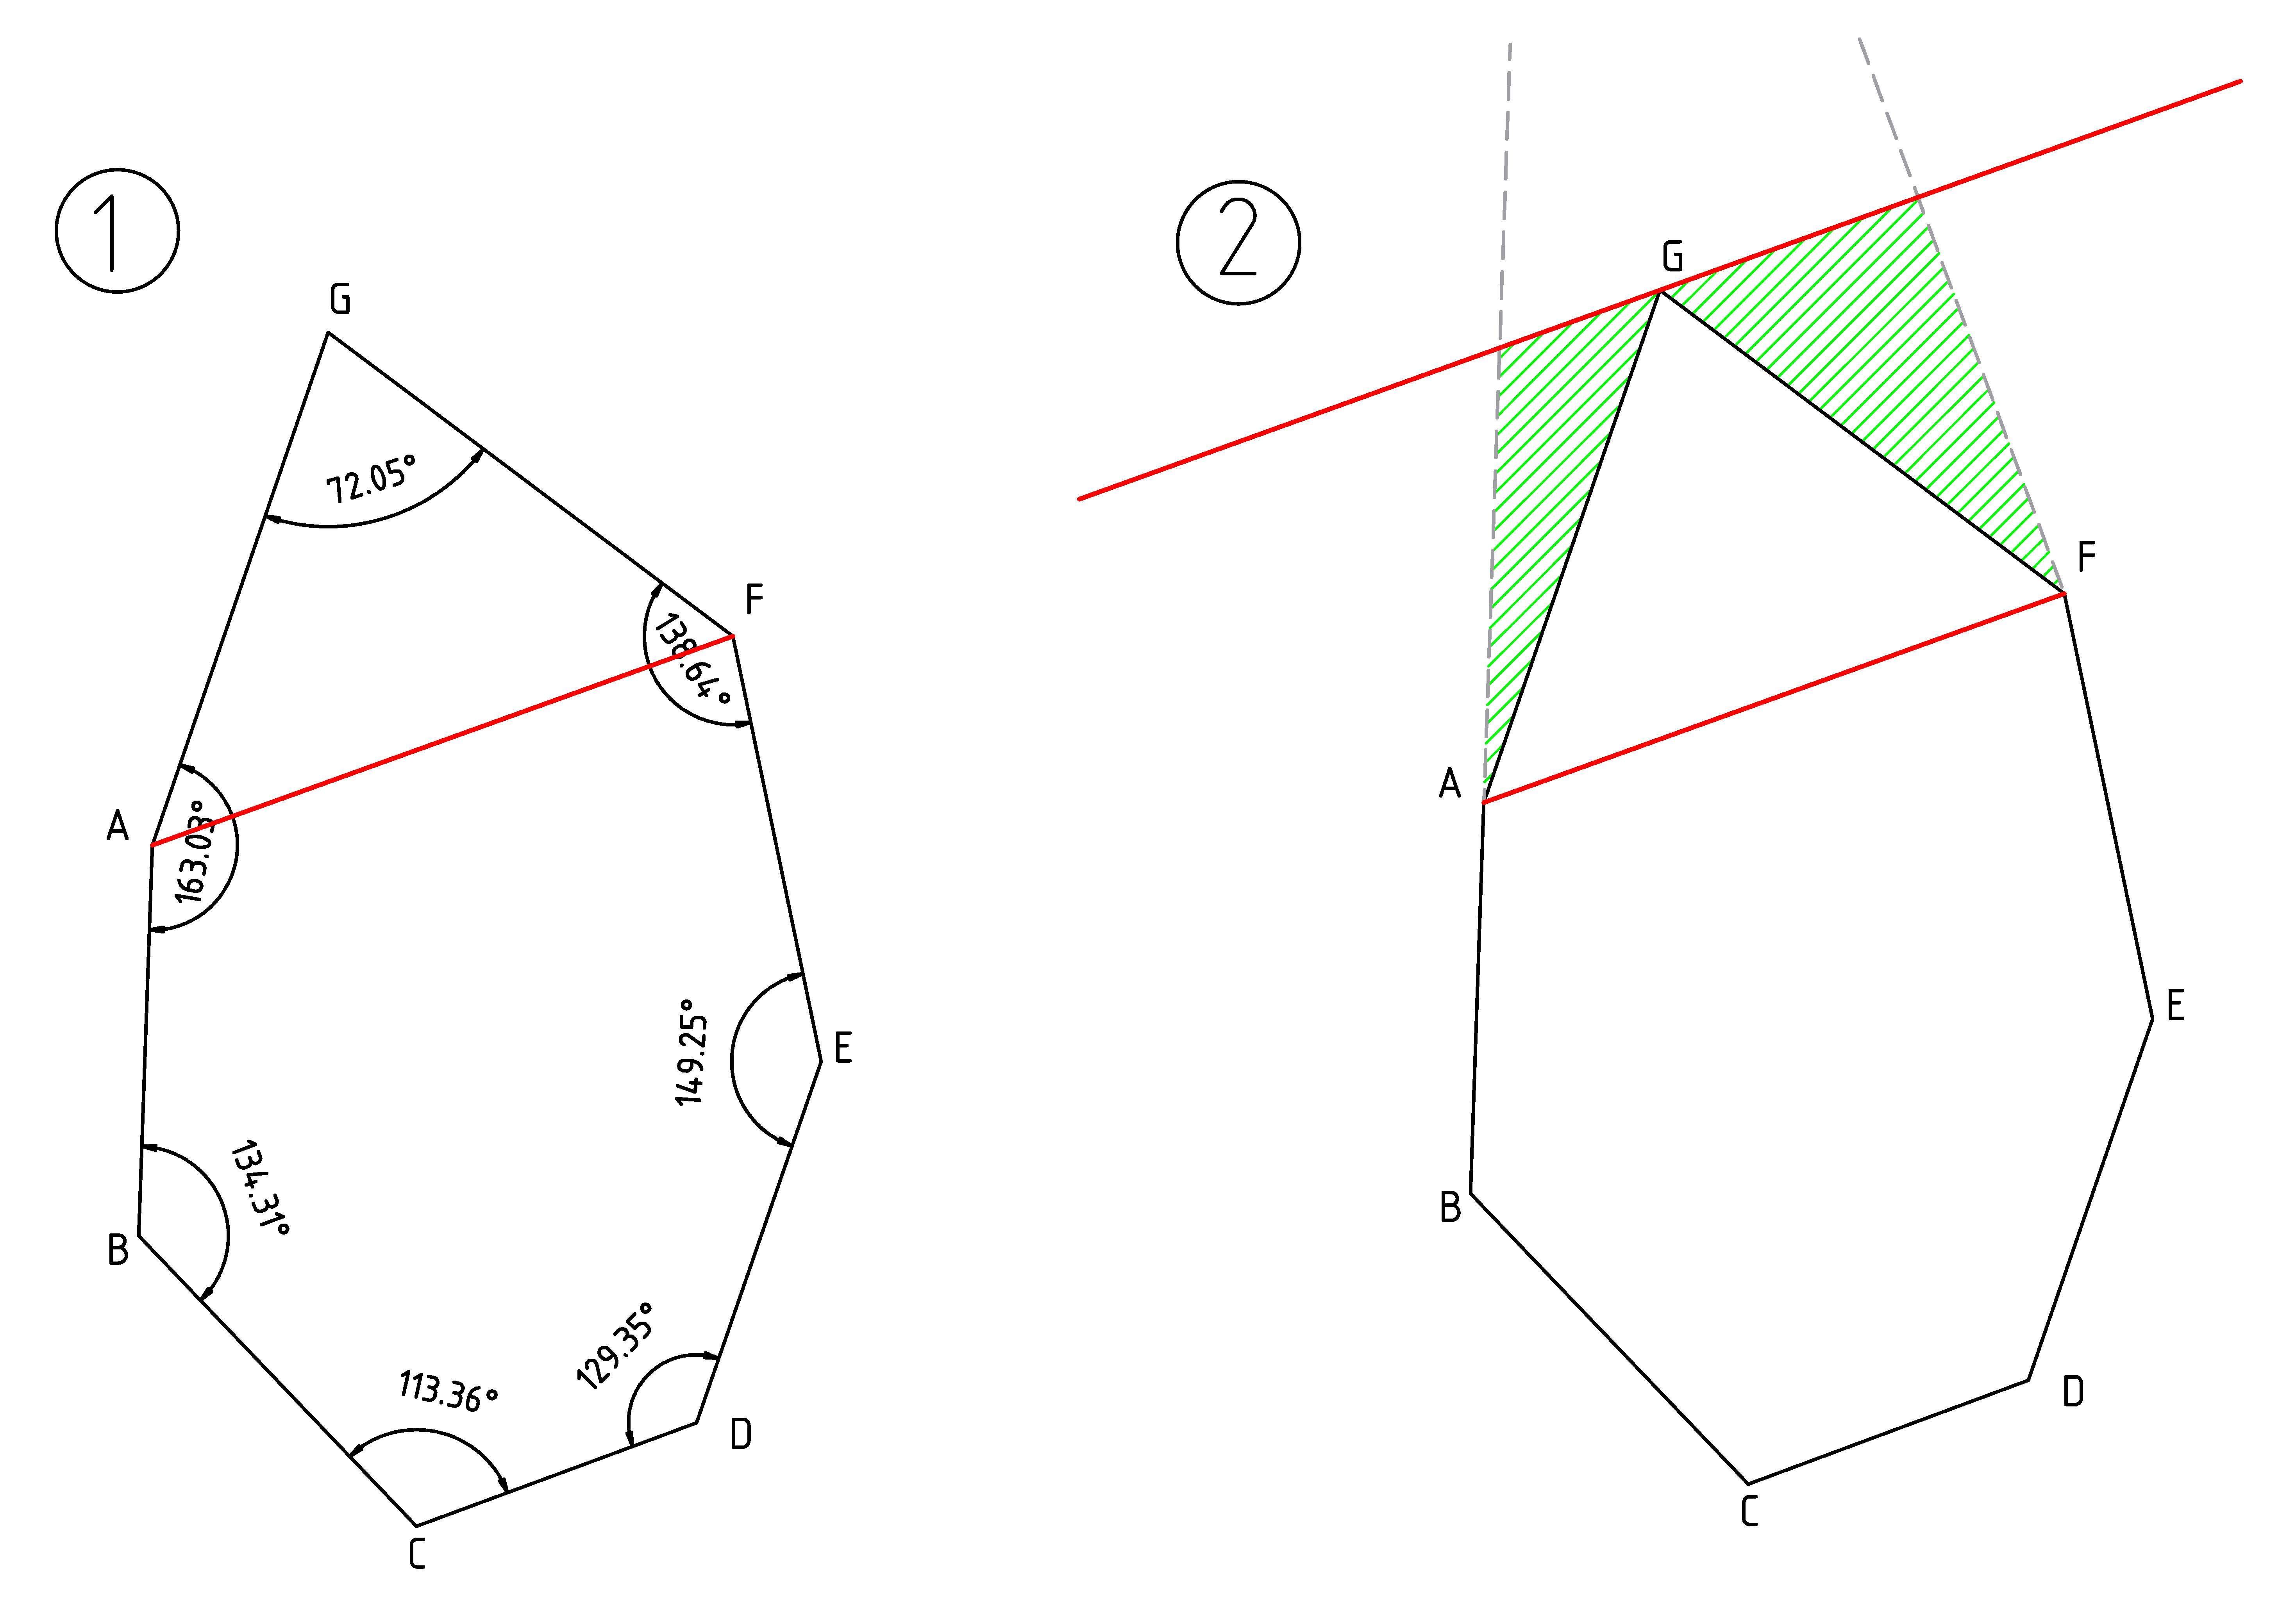
\includegraphics[width=0.8\textwidth]{media/Demo_algorithms/demo_smaller_angle.jpg} \\
        \begin{tabular}{l}
            (1) Creazione di un iperpiano secondo CSA \\
            (2) Traslazione dell'iperpiano creato secondo CSA2
        \end{tabular}
    \end{tabular}
\end{figure}

\begin{center}
    Esempi di approssimazione:
\end{center}
\begin{figure}[H]
    \centering
    \begin{tabular}{ccc}
        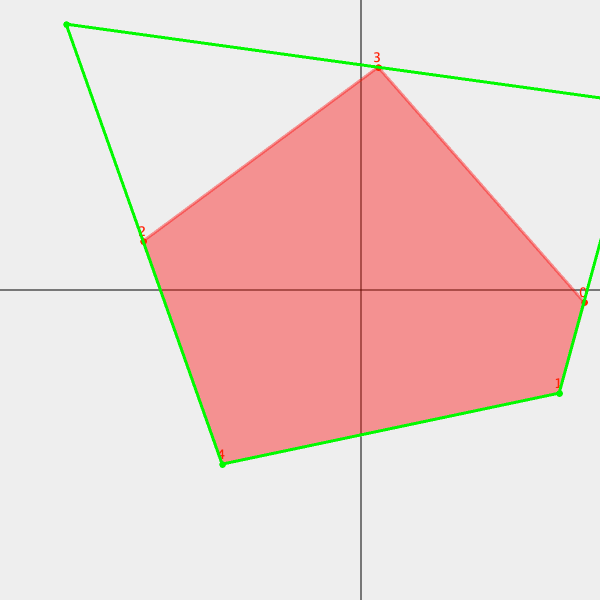
\includegraphics[width=0.3\textwidth]{media/CuttingSmallerAngle2/5_4.png} &
        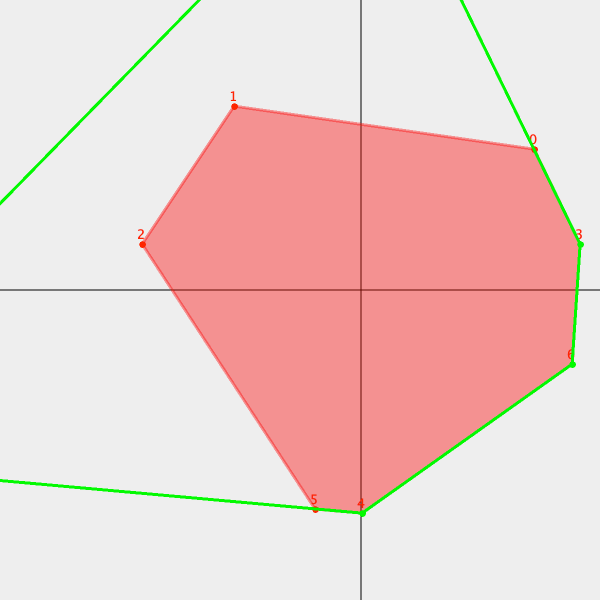
\includegraphics[width=0.3\textwidth]{media/CuttingSmallerAngle2/7_5.png} &
        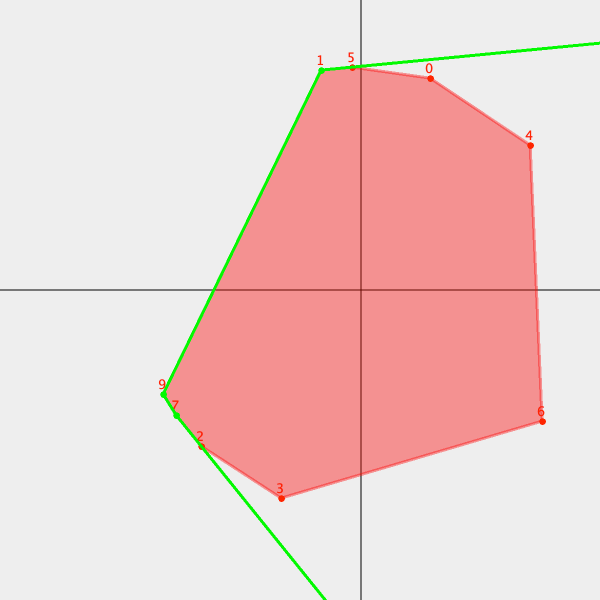
\includegraphics[width=0.3\textwidth]{media/CuttingSmallerAngle2/9_5.png} \\
        (a) E = 5, h = 4 & (b) E = 7, h = 5 & (c) E = 9, h = 5
    \end{tabular}
\end{figure}

Questo approccio rende l'algoritmo precedente accettabile poichè rispetta l'inclusione
dell'area ammissibile di partenza. Tuttavia, all'aumentare dei vertici, è molto probabile 
che un numero eccessivo di traslazioni interessino un iperpiano. questo porterebbe
alla deriva il lato rendendo, così il volume del politopo risultante eccessivo 
rispetto all'originale (come si può verificare dagli esempi (b) e (c)).


\pagebreak
\subsection{Ipotesi di Algoritmo Cutting Larger Angle (CLA)}

Utilizzando un approccio inverso all'algoritmo CSA, si potrebbe ipotizzare che gli angoli interni 
con ampiezza maggiore siano i candidati migliori per essere approssimati con un segmento, 
poichè la perdita di volume, una volta applicato il taglio, sarebbe la piu piccola possibile.

\begin{center}
    Esempi di approssimazione:
\end{center}
\begin{figure}[H]
    \centering
    \begin{tabular}{ccc}
        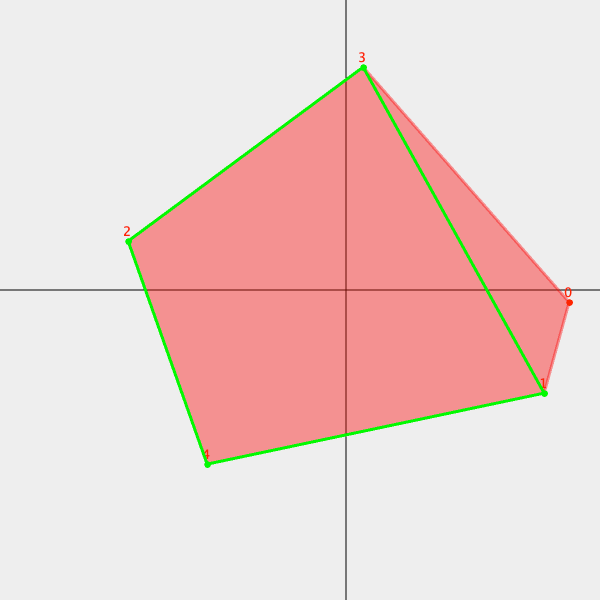
\includegraphics[width=0.3\textwidth]{media/CuttingLargerAngle/5_4.png} &
        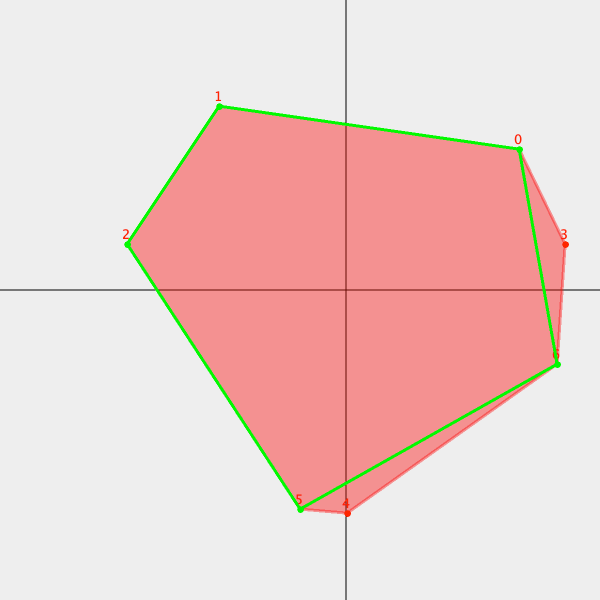
\includegraphics[width=0.3\textwidth]{media/CuttingLargerAngle/7_5.png} &
        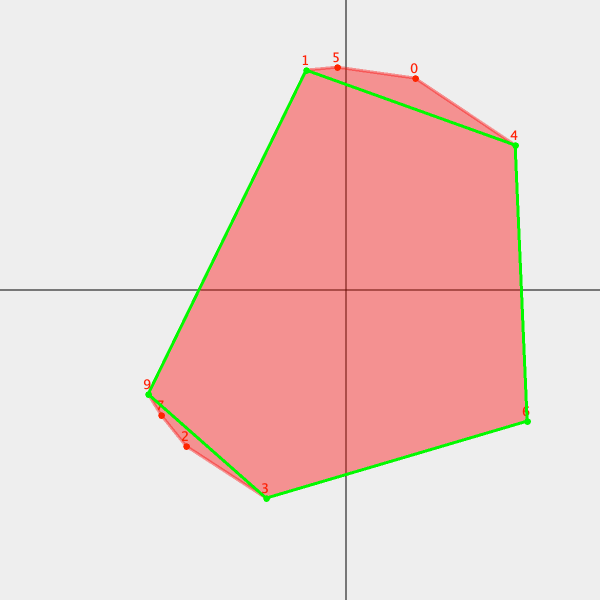
\includegraphics[width=0.3\textwidth]{media/CuttingLargerAngle/9_5.png} \\
        (a) E = 5, h = 4 & (b) E = 7, h = 5 & (c) E = 9, h = 5
    \end{tabular}
\end{figure}

Si rivela un approccio vincente in termini di somiglianza con l'area del guscio convesso di partenza, 
ma condivide con l'approccio CSA il fatto di non includere i nodi che vengono tagliati,
rendendolo così inaccettabile.

\pagebreak
\subsection{Ipotesi di Algoritmo Cutting Larger Angle 2 (CLA2)}

Applicando la medesima trasformazione applicata all'algoritmo CSA, si consente al precedente 
algoritmo di includere tutti i punti ammissibili, rendendo di fatto il precedente algoritmo accettabile.

\begin{figure}[H]
    \centering
    \begin{tabular}{c}
        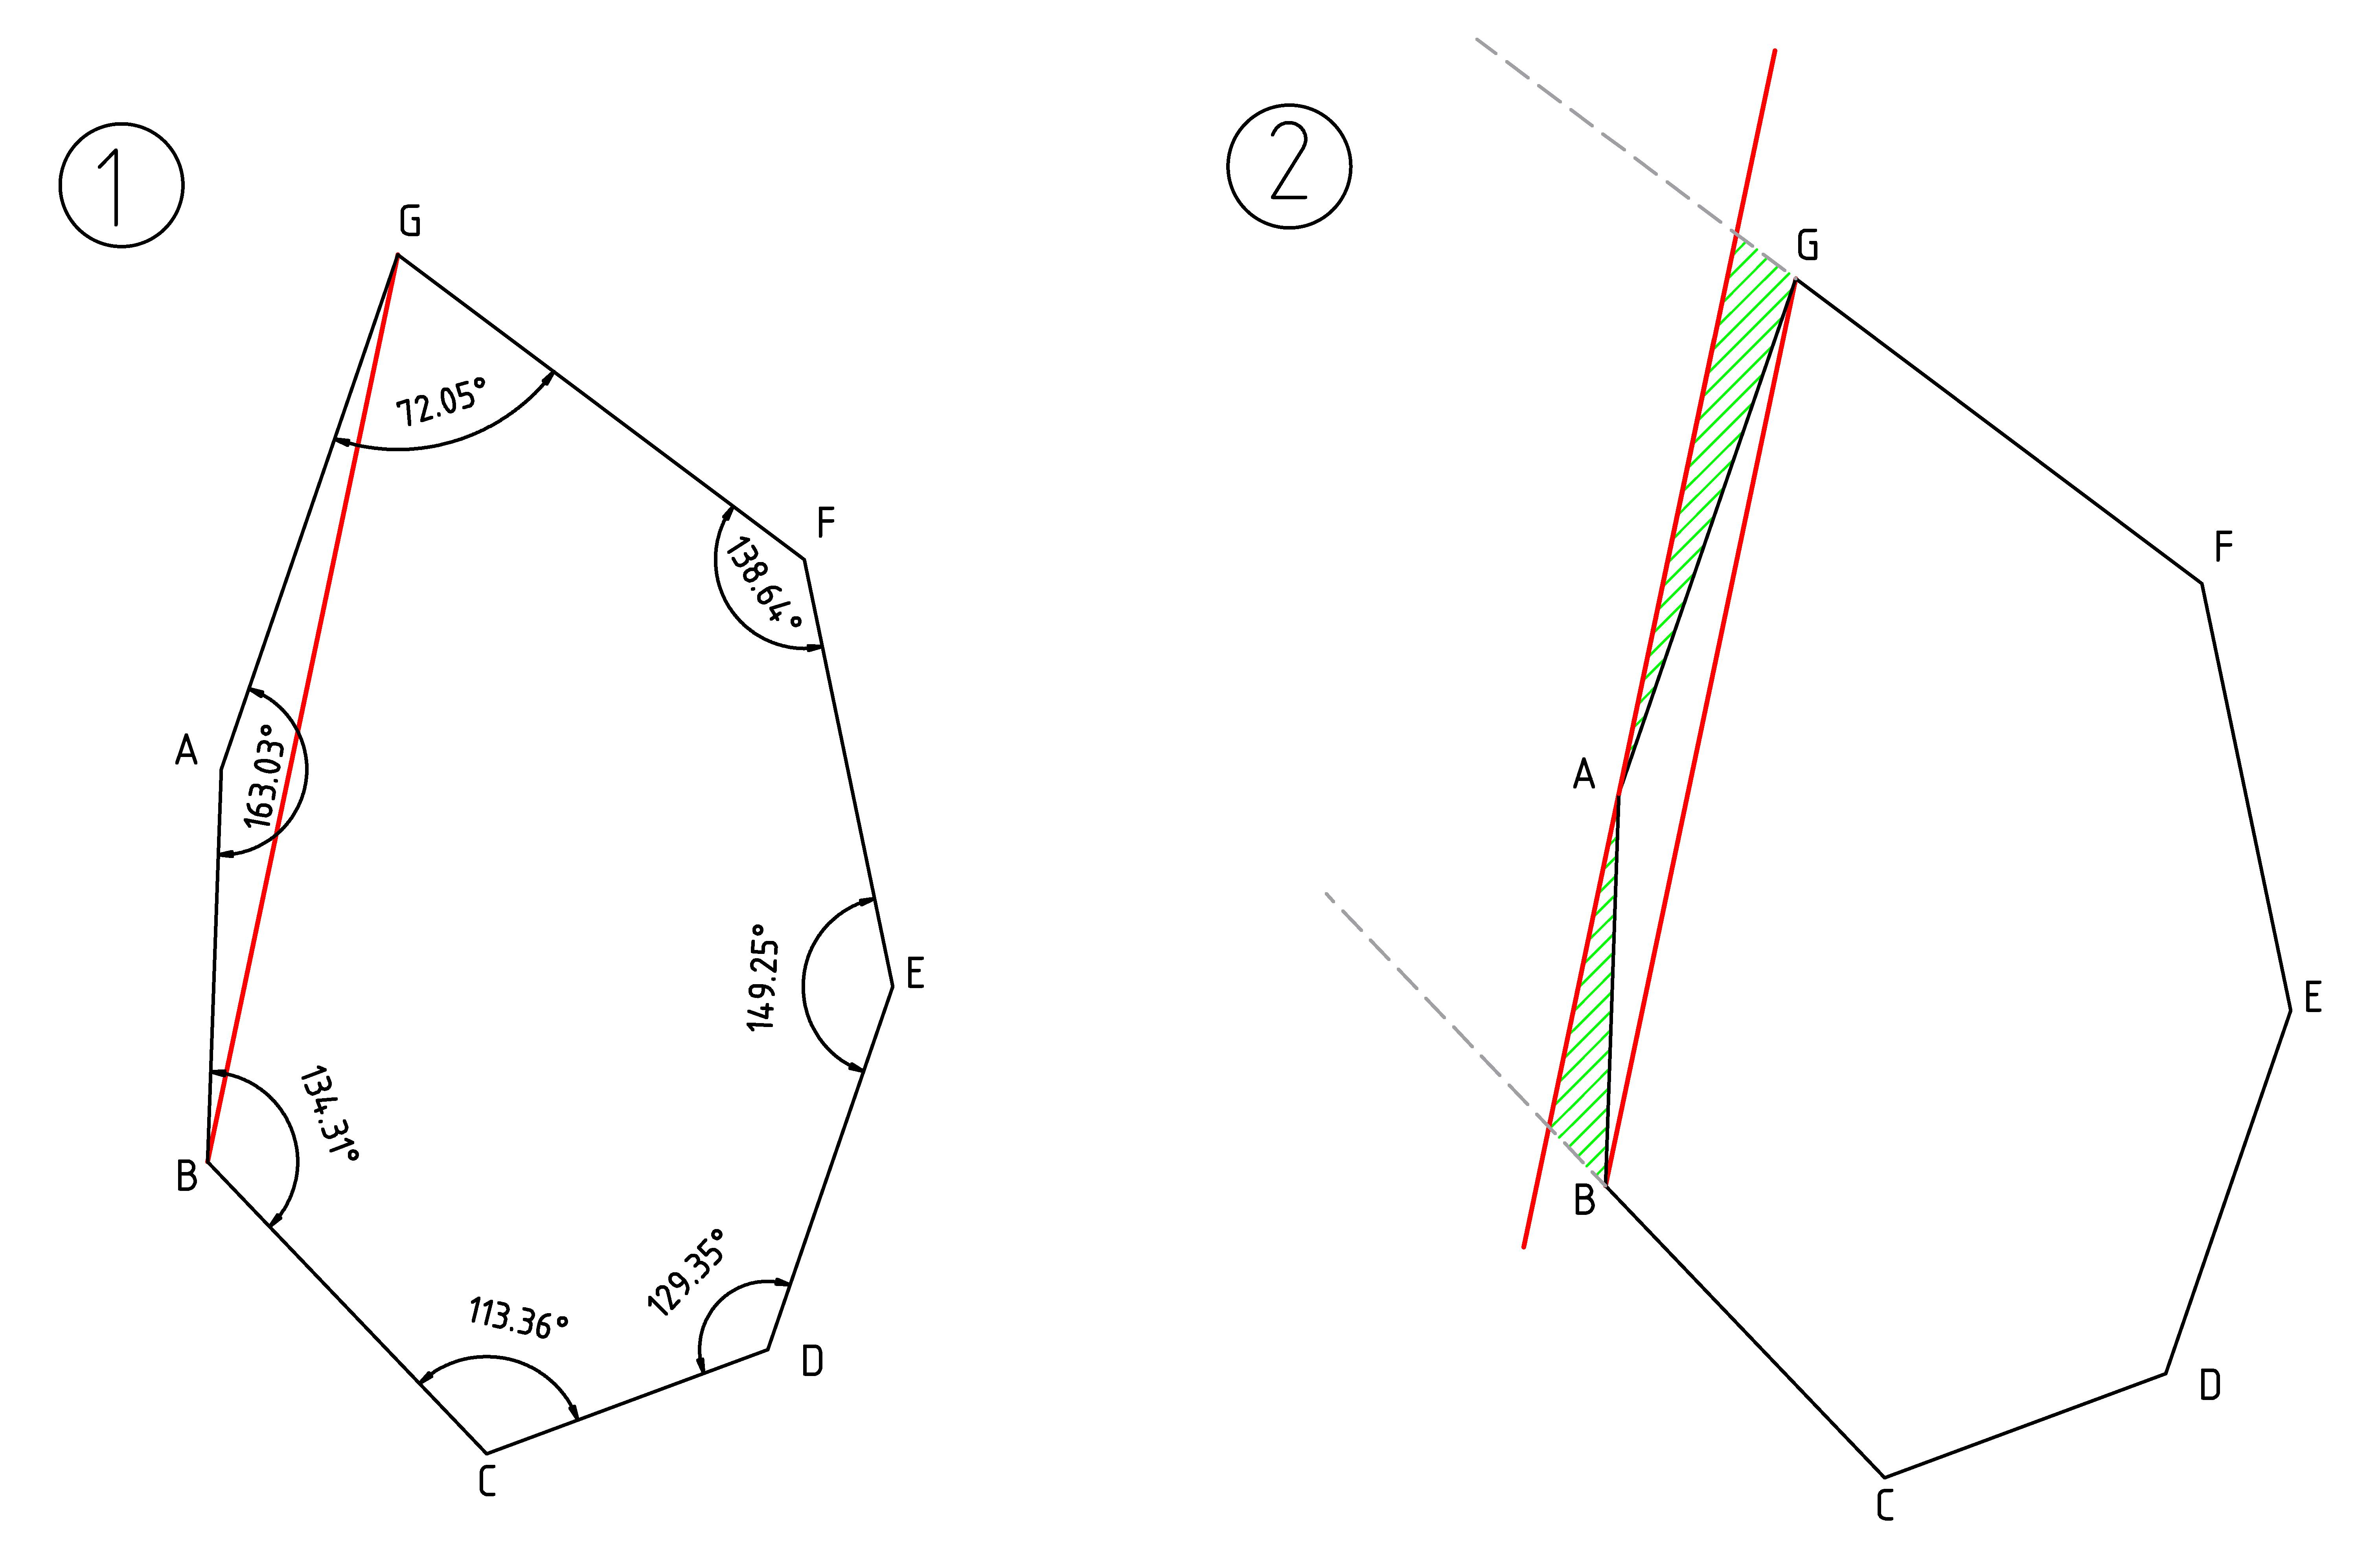
\includegraphics[width=0.8\textwidth]{media/Demo_algorithms/demo_larger_angle.jpg} \\
        \begin{tabular}{l}
            (1) Creazione di un iperpiano secondo CLA \\
            (2) Traslazione dell'iperpiano creato secondo CLA2
        \end{tabular}
    \end{tabular}
\end{figure}

\begin{center}
    Esempi di approssimazione:
\end{center}
\begin{figure}[H]
    \centering
    \begin{tabular}{ccc}
        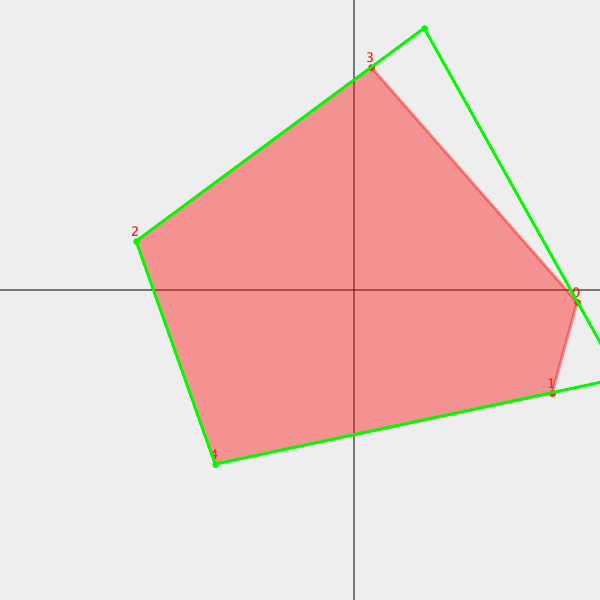
\includegraphics[width=0.3\textwidth]{media/CuttingLargerAngle2/5_4.png} &
        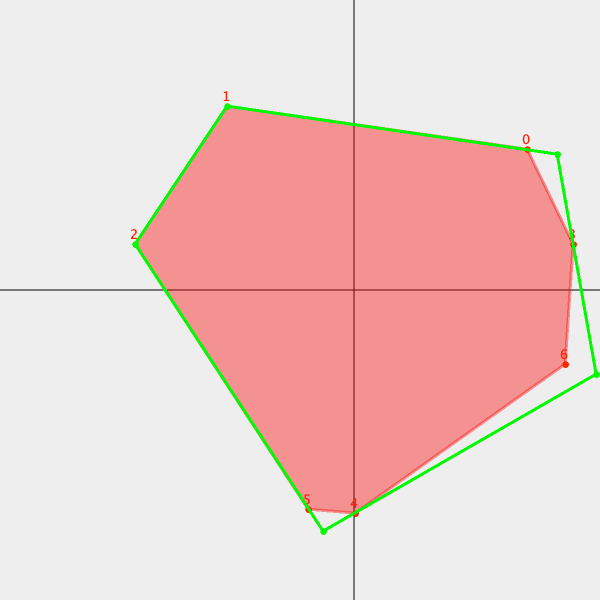
\includegraphics[width=0.3\textwidth]{media/CuttingLargerAngle2/7_5.png} &
        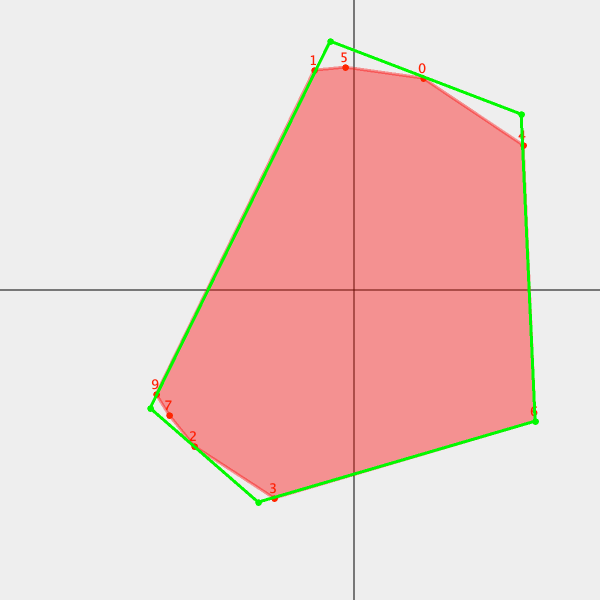
\includegraphics[width=0.3\textwidth]{media/CuttingLargerAngle2/9_5.png} \\
        (a) e = 5, h = 4 & (b) e = 7, h = 5 & (c) e = 9, h = 5
    \end{tabular}
\end{figure}

Il risultato ottenuto, in termini di somiglianza visiva con il poligono originale, è buono. 
A rafforzare questo punto viene anche il rispettivo indice di Jaccard analizzato nella sezione 
\hyperref[sec:Analisi dei dati]{Analisi dei dati}.

\pagebreak
\subsection{Ipotesi di Algoritmo Distance From G (DFG)}

Questo algoritmo prevede la ricerca dei vertici più distanti dal baricentro del guscio convesso. 
Una volta selezionati $h$ vertici, viene costruito il poligono risultante.
Successivamente ogni lato che esclude vertici del poliedro originale viene traslato fino al 
loro contenimento.\\

Onde evitare che un numero elevato di vertici concentrati in una regione limitata del guscio convesso
influenzino il calcolo del baricentro calcolato con la formula 
\[
G_i = \frac{1}{n} \sum_{k=1}^{n} x_{k,i}
\]
si procede a considerare come baricentro della regione ammissibile il centro di massa 
della corrispettiva \textit{bounding box}.\\

\begin{figure}[H]
    \centering
    \begin{tabular}{c}
        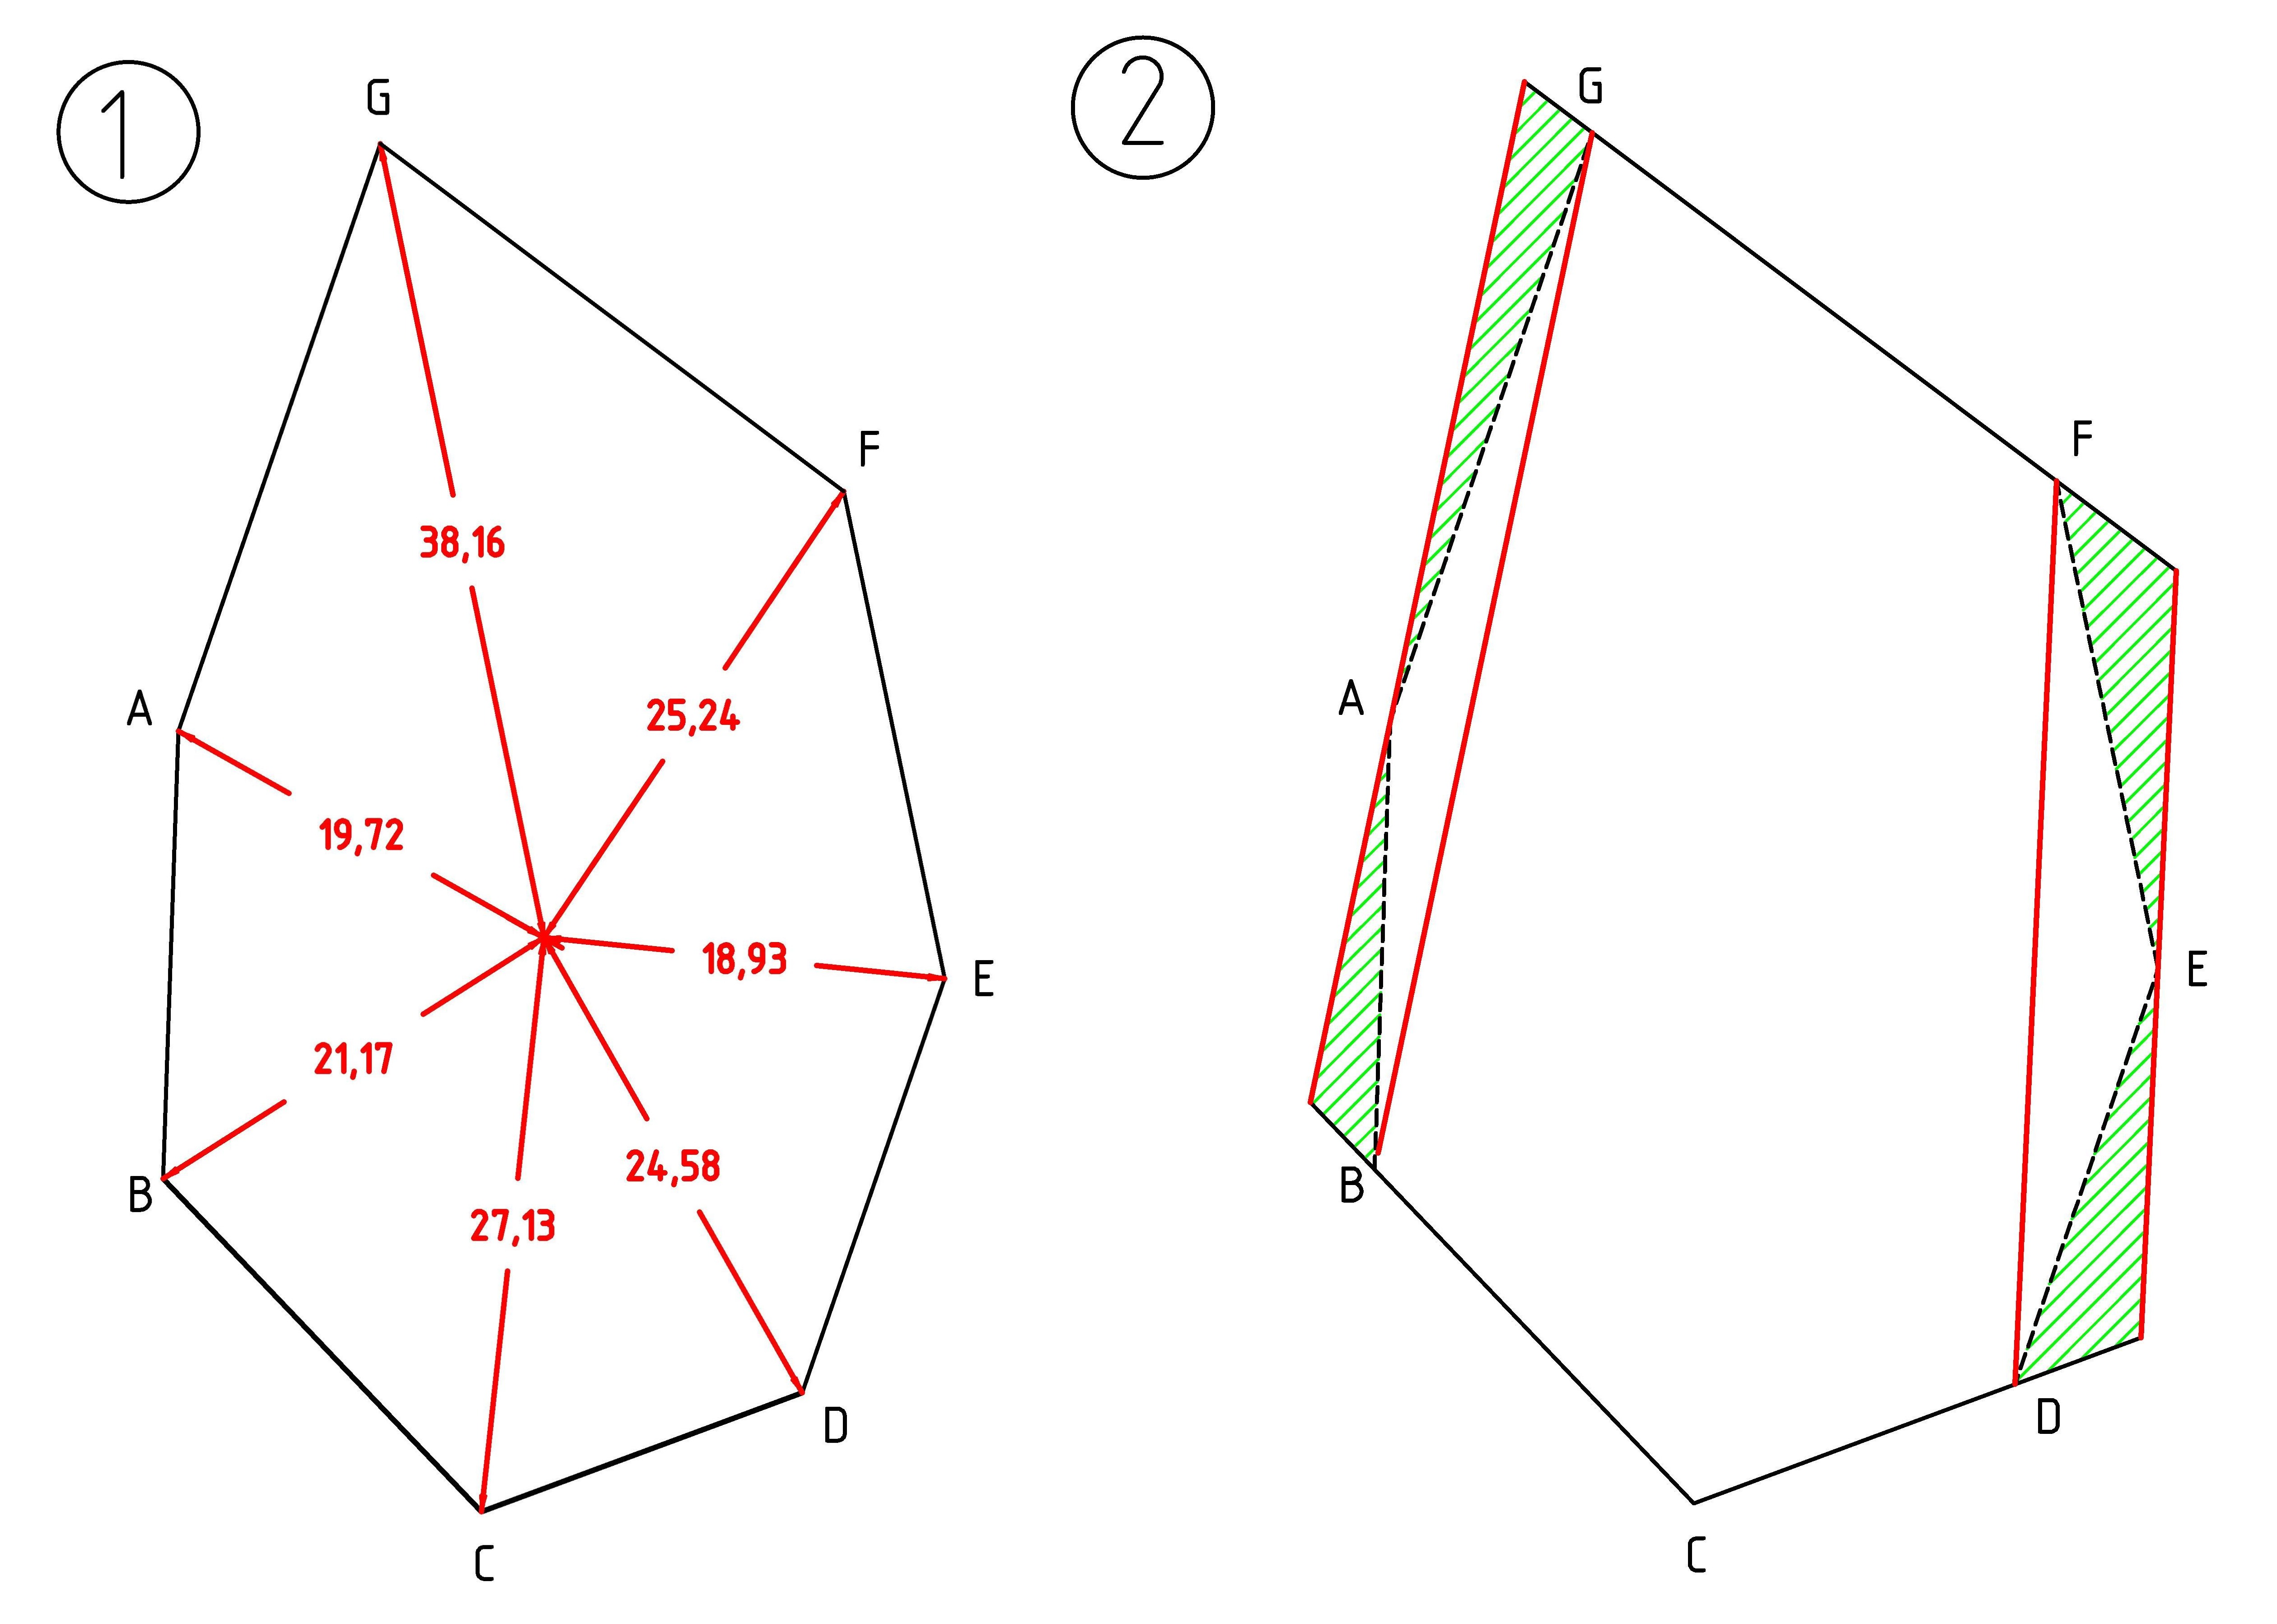
\includegraphics[width=0.8\textwidth]{media/Demo_algorithms/demo_distance_g.jpg} \\
        \begin{tabular}{l}
            (1) Dimostrazione del criterio di scelta dei vertici secondo DFG\\
            (2) Traslazione degli iperpiani interni dell'approssimazione secondo DFG
        \end{tabular}
    \end{tabular}
\end{figure}

\begin{center}
    Esempi di approssimazione:
\end{center}
\begin{figure}[H]
    \centering
    \begin{tabular}{ccc}
        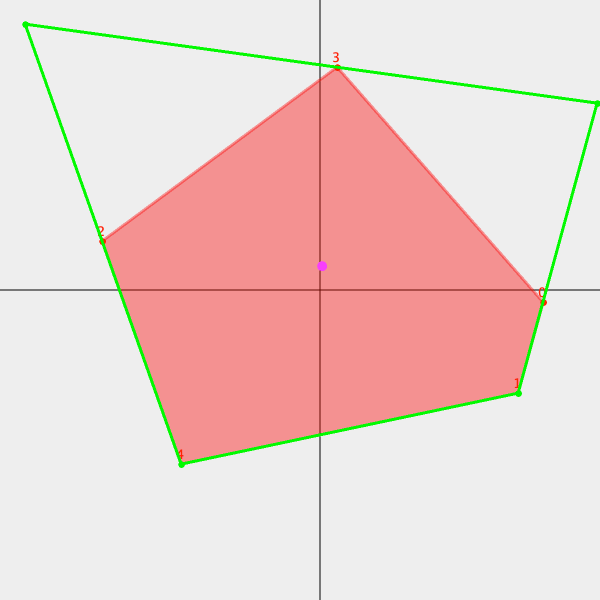
\includegraphics[width=0.3\textwidth]{media/DistanceFromG/5_4.png} &
        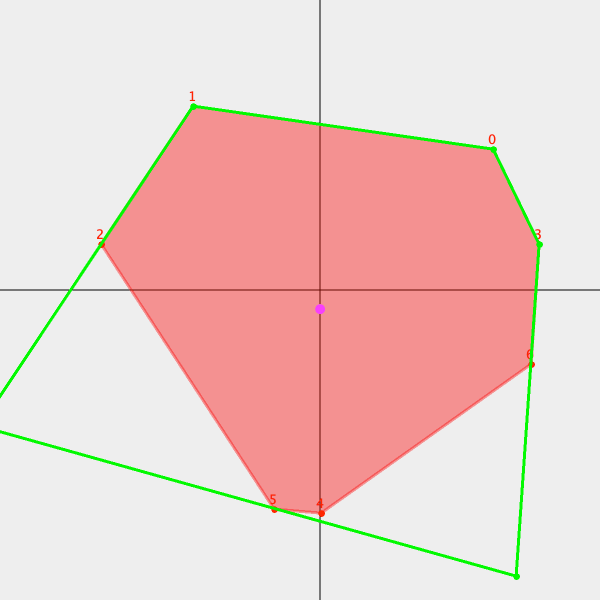
\includegraphics[width=0.3\textwidth]{media/DistanceFromG/7_5.png} &
        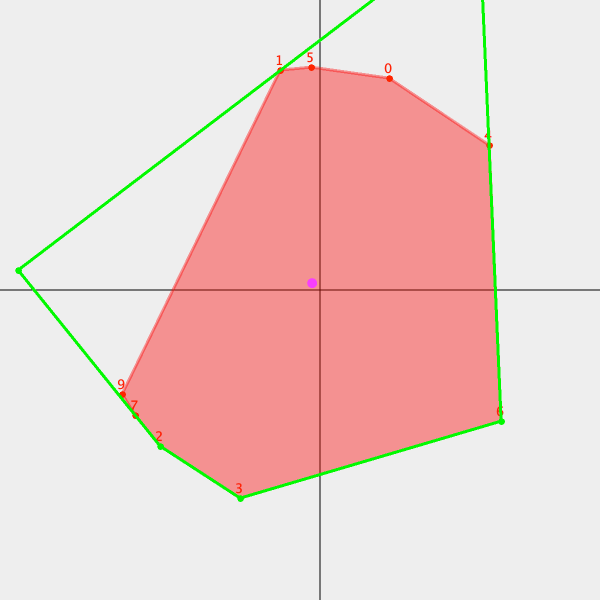
\includegraphics[width=0.3\textwidth]{media/DistanceFromG/9_5.png} \\
        (a) E = 5, h = 4 & (b) E = 7, h = 5 & (c) E = 9, h = 5
    \end{tabular}
\end{figure}

\pagebreak
\section{Approssimazioni tramite analisi delle proprietà degli iperpiani}

A differenza dei precedenti, gli algoritmi illustrati di seguito analizzano proprietà
intrinseche degli iperpiani del guscio convesso (come volumi eccedenti o aree proiettate),
selezionando un numero di iperpiani congruo al budget fornito secondo differenti criteri.
Questa caratteristica garantisce che, in un qualunque passaggio di computazione, 
il politopo approssimativo non escluda mai parti della regione ammissibile di partenza.

\subsection{Ipotesi di Algoritmo BoxCutting}

L'algoritmo prende direttamente in considerazione la \textit{Bounding Box} del 
politopo originale per poter effettuare dei tagli al volume di questa in modo tale 
che, con ognuno di questi, il volume generato dagli iperpiani di taglio arrivi a 
combaciare con quello originale.
Per sua natura utilizza un approccio inverso agli altri algoritmi della categoria 
poichè, a partire da un poliedro più semplice, si converge verso il politopo originale.

\begin{figure}[H]
    \centering
    \begin{tabular}{c}
        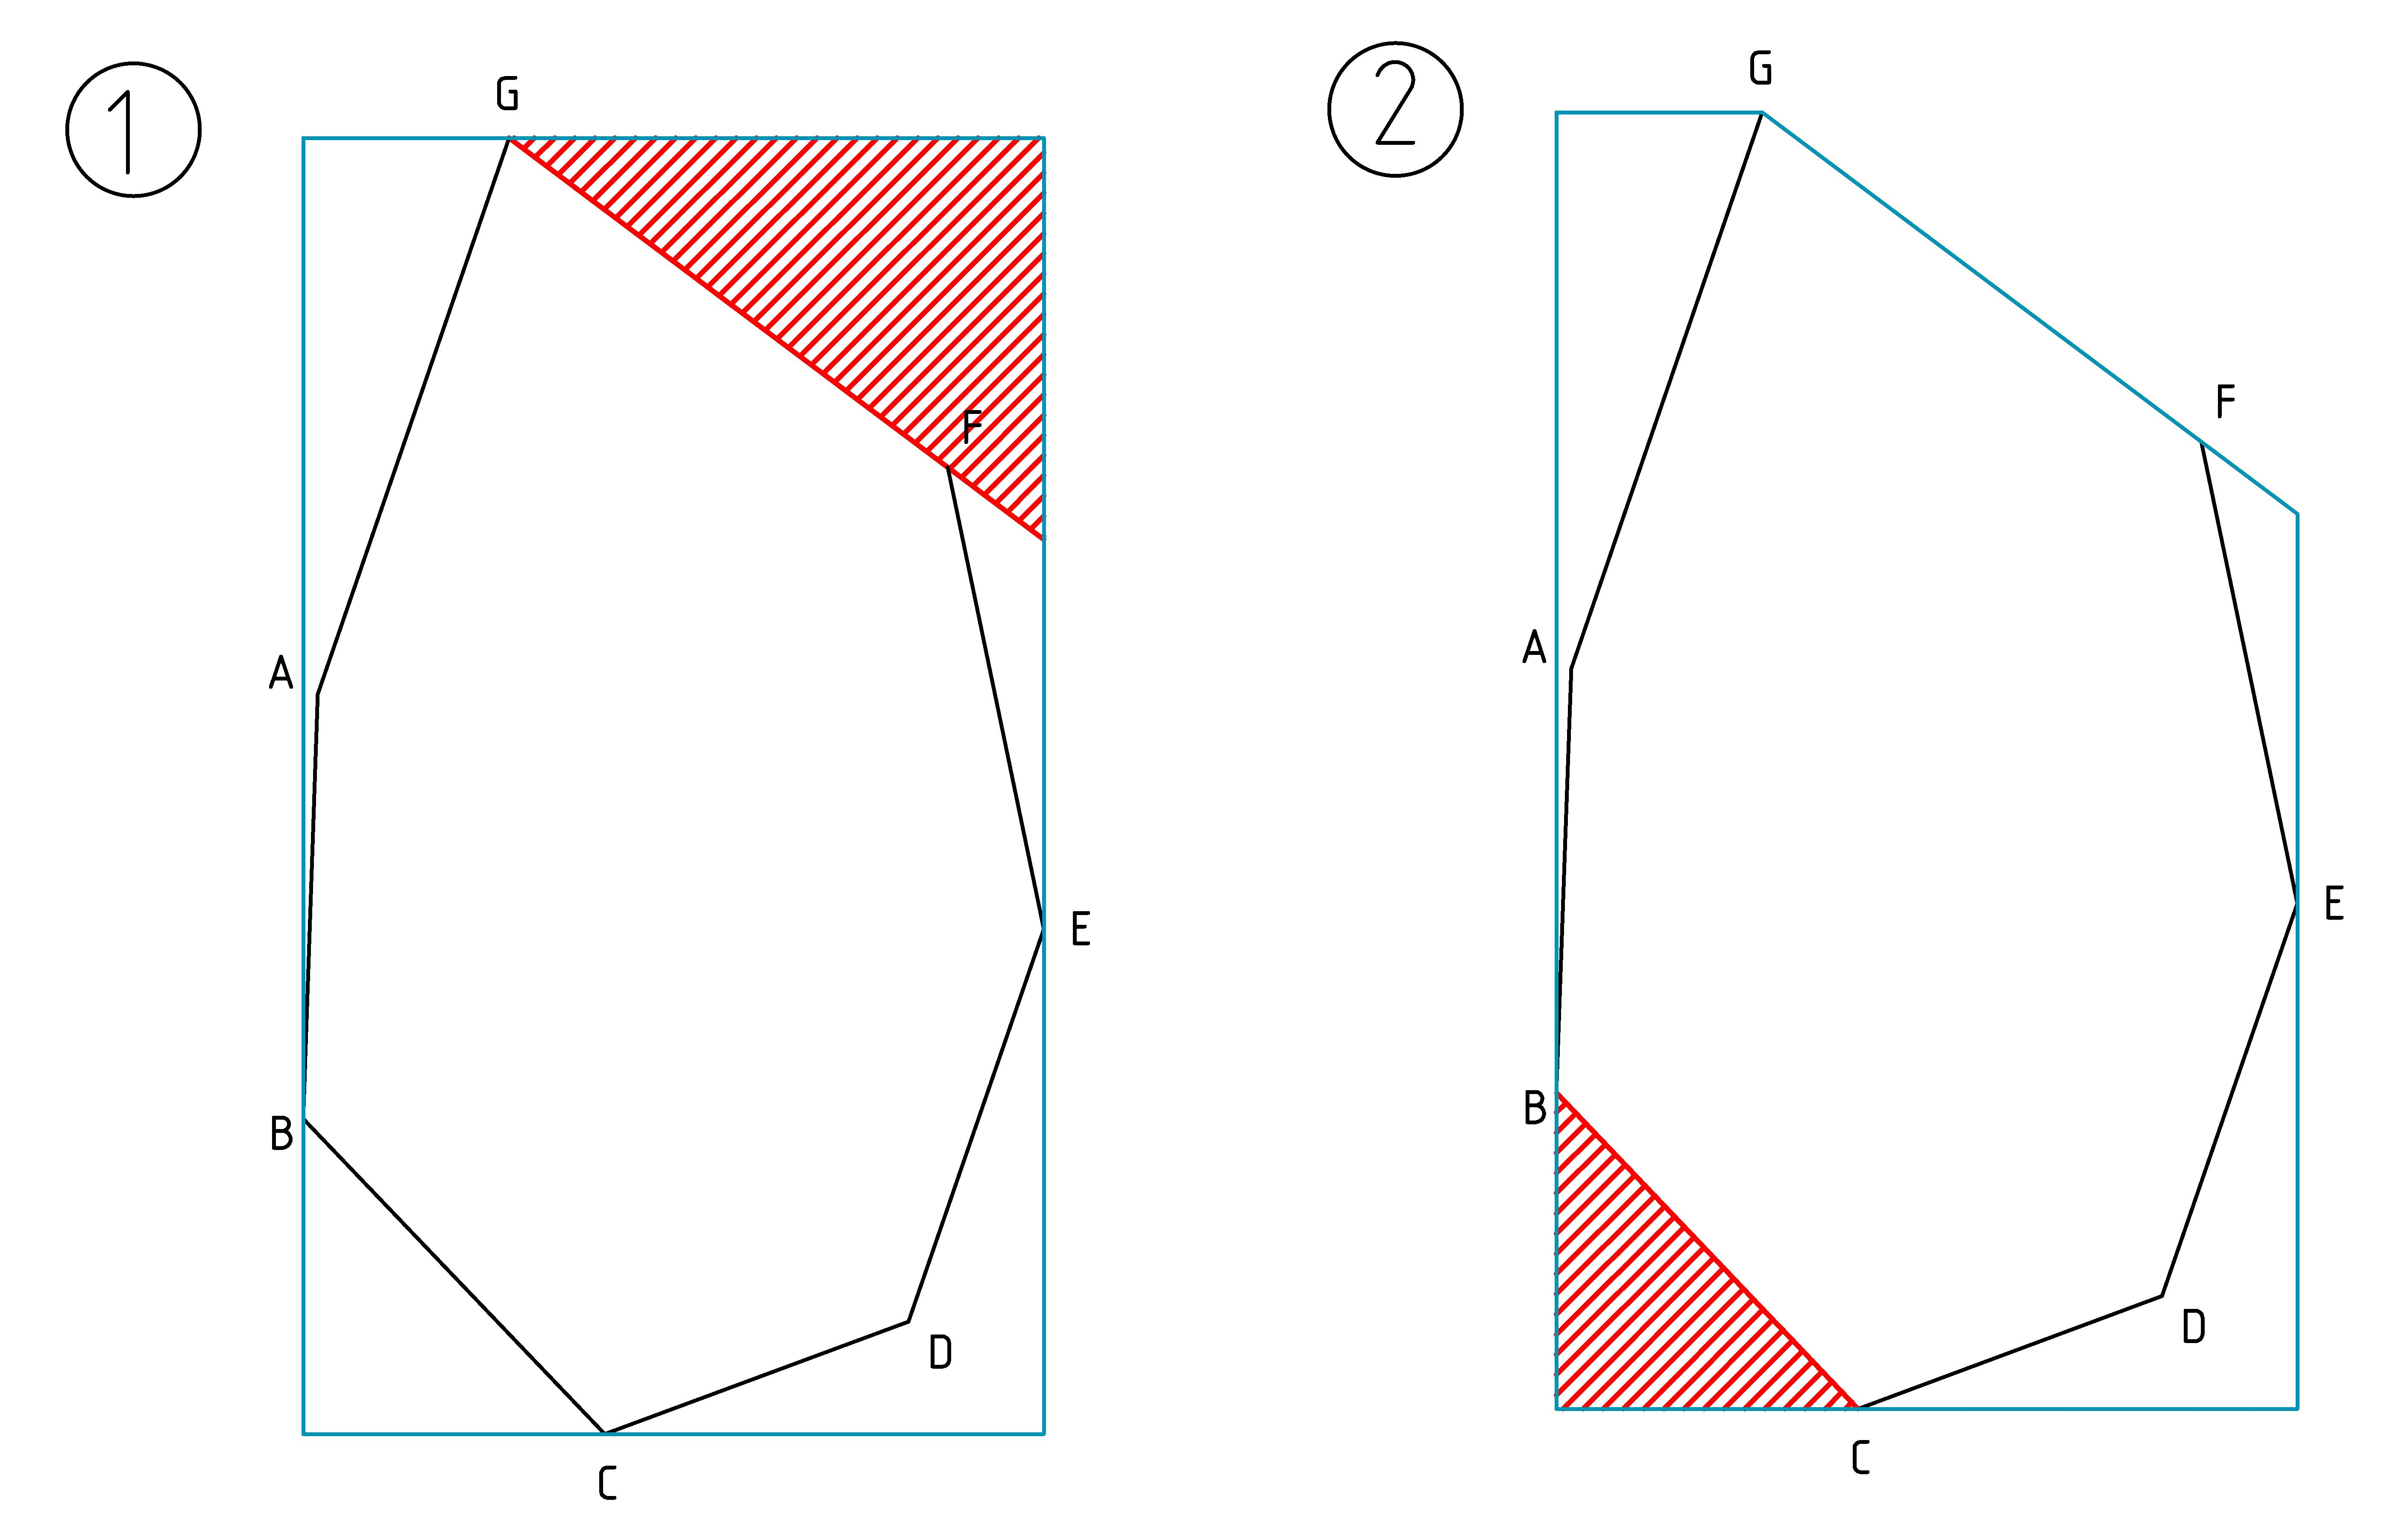
\includegraphics[width=0.8\textwidth]{media/Demo_algorithms/demo_box_cutting.jpg} \\
        \begin{tabular}{l}
            (1) Dimostrazione del criterio di scelta dell'iperpiano migliore secondo B.C.\\
            (2) Dimostrazione del criterio di scelta sul restante politopo
        \end{tabular}
    \end{tabular}
\end{figure}

\begin{center}
    Esempi di approssimazione:
\end{center}
\begin{figure}[H]
    \centering
    \begin{tabular}{ccc}
        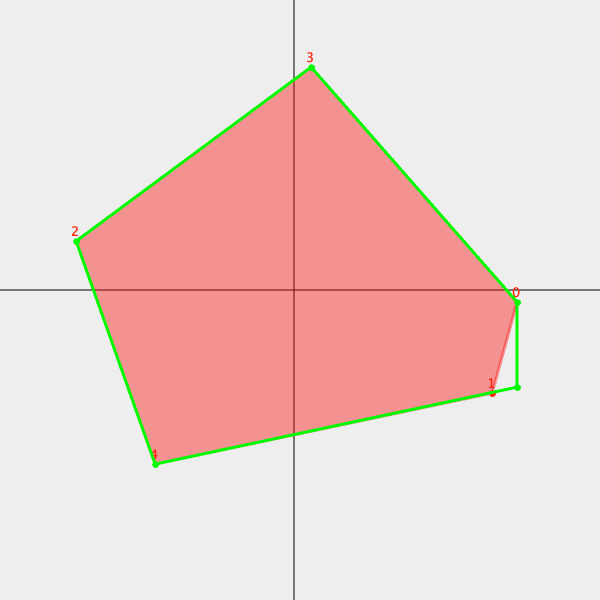
\includegraphics[width=0.3\textwidth]{media/BoxCutting/5_4.png} &
        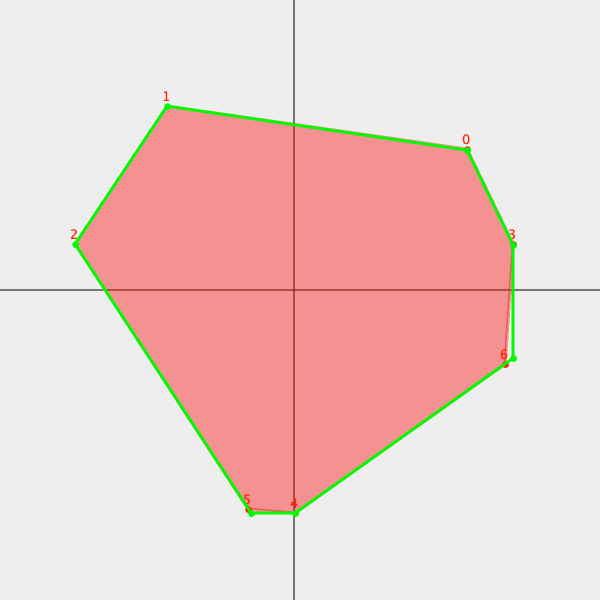
\includegraphics[width=0.3\textwidth]{media/BoxCutting/7_5.png} &
        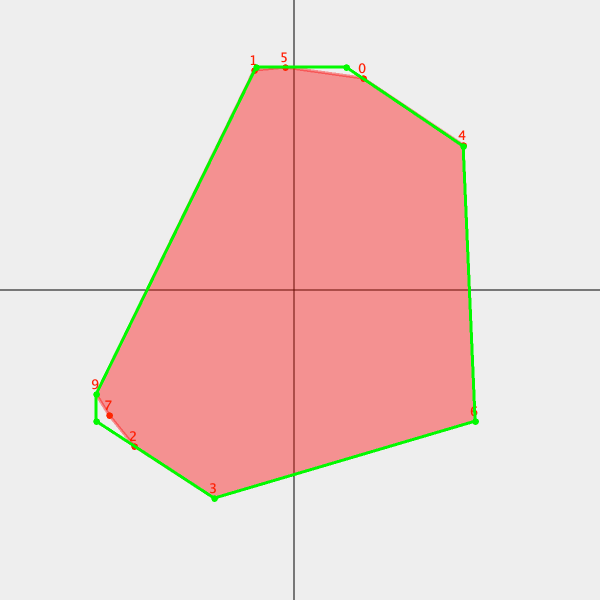
\includegraphics[width=0.3\textwidth]{media/BoxCutting/9_5.png} \\
        (a) E = 5, h = 4 & (b) E = 7, h = 5 & (c) E = 9, h = 5
    \end{tabular}
\end{figure}

L'approccio unico utilizzato offre diversi vantaggi, quali l'ottenimento di una approssimazione
con pochi iperpiani del politopo originale sin dalle prime iterazioni.
L'approssimazione diventa di fatti progressivamente costosa computazionalmente al crescere
di $h$.


\subsection{Ipotesi di Algoritmo Less Area}

L'algoritmo ipotizzato cerca i lati che meglio possano rappresentare un lato del poligono 
selezionando gli iperpiani che tendono a minimizzare l'area compresa fra essi e il poligono stesso, 
come mostrato in figura.

\begin{figure}[H]
    \centering
    \begin{tabular}{c}
        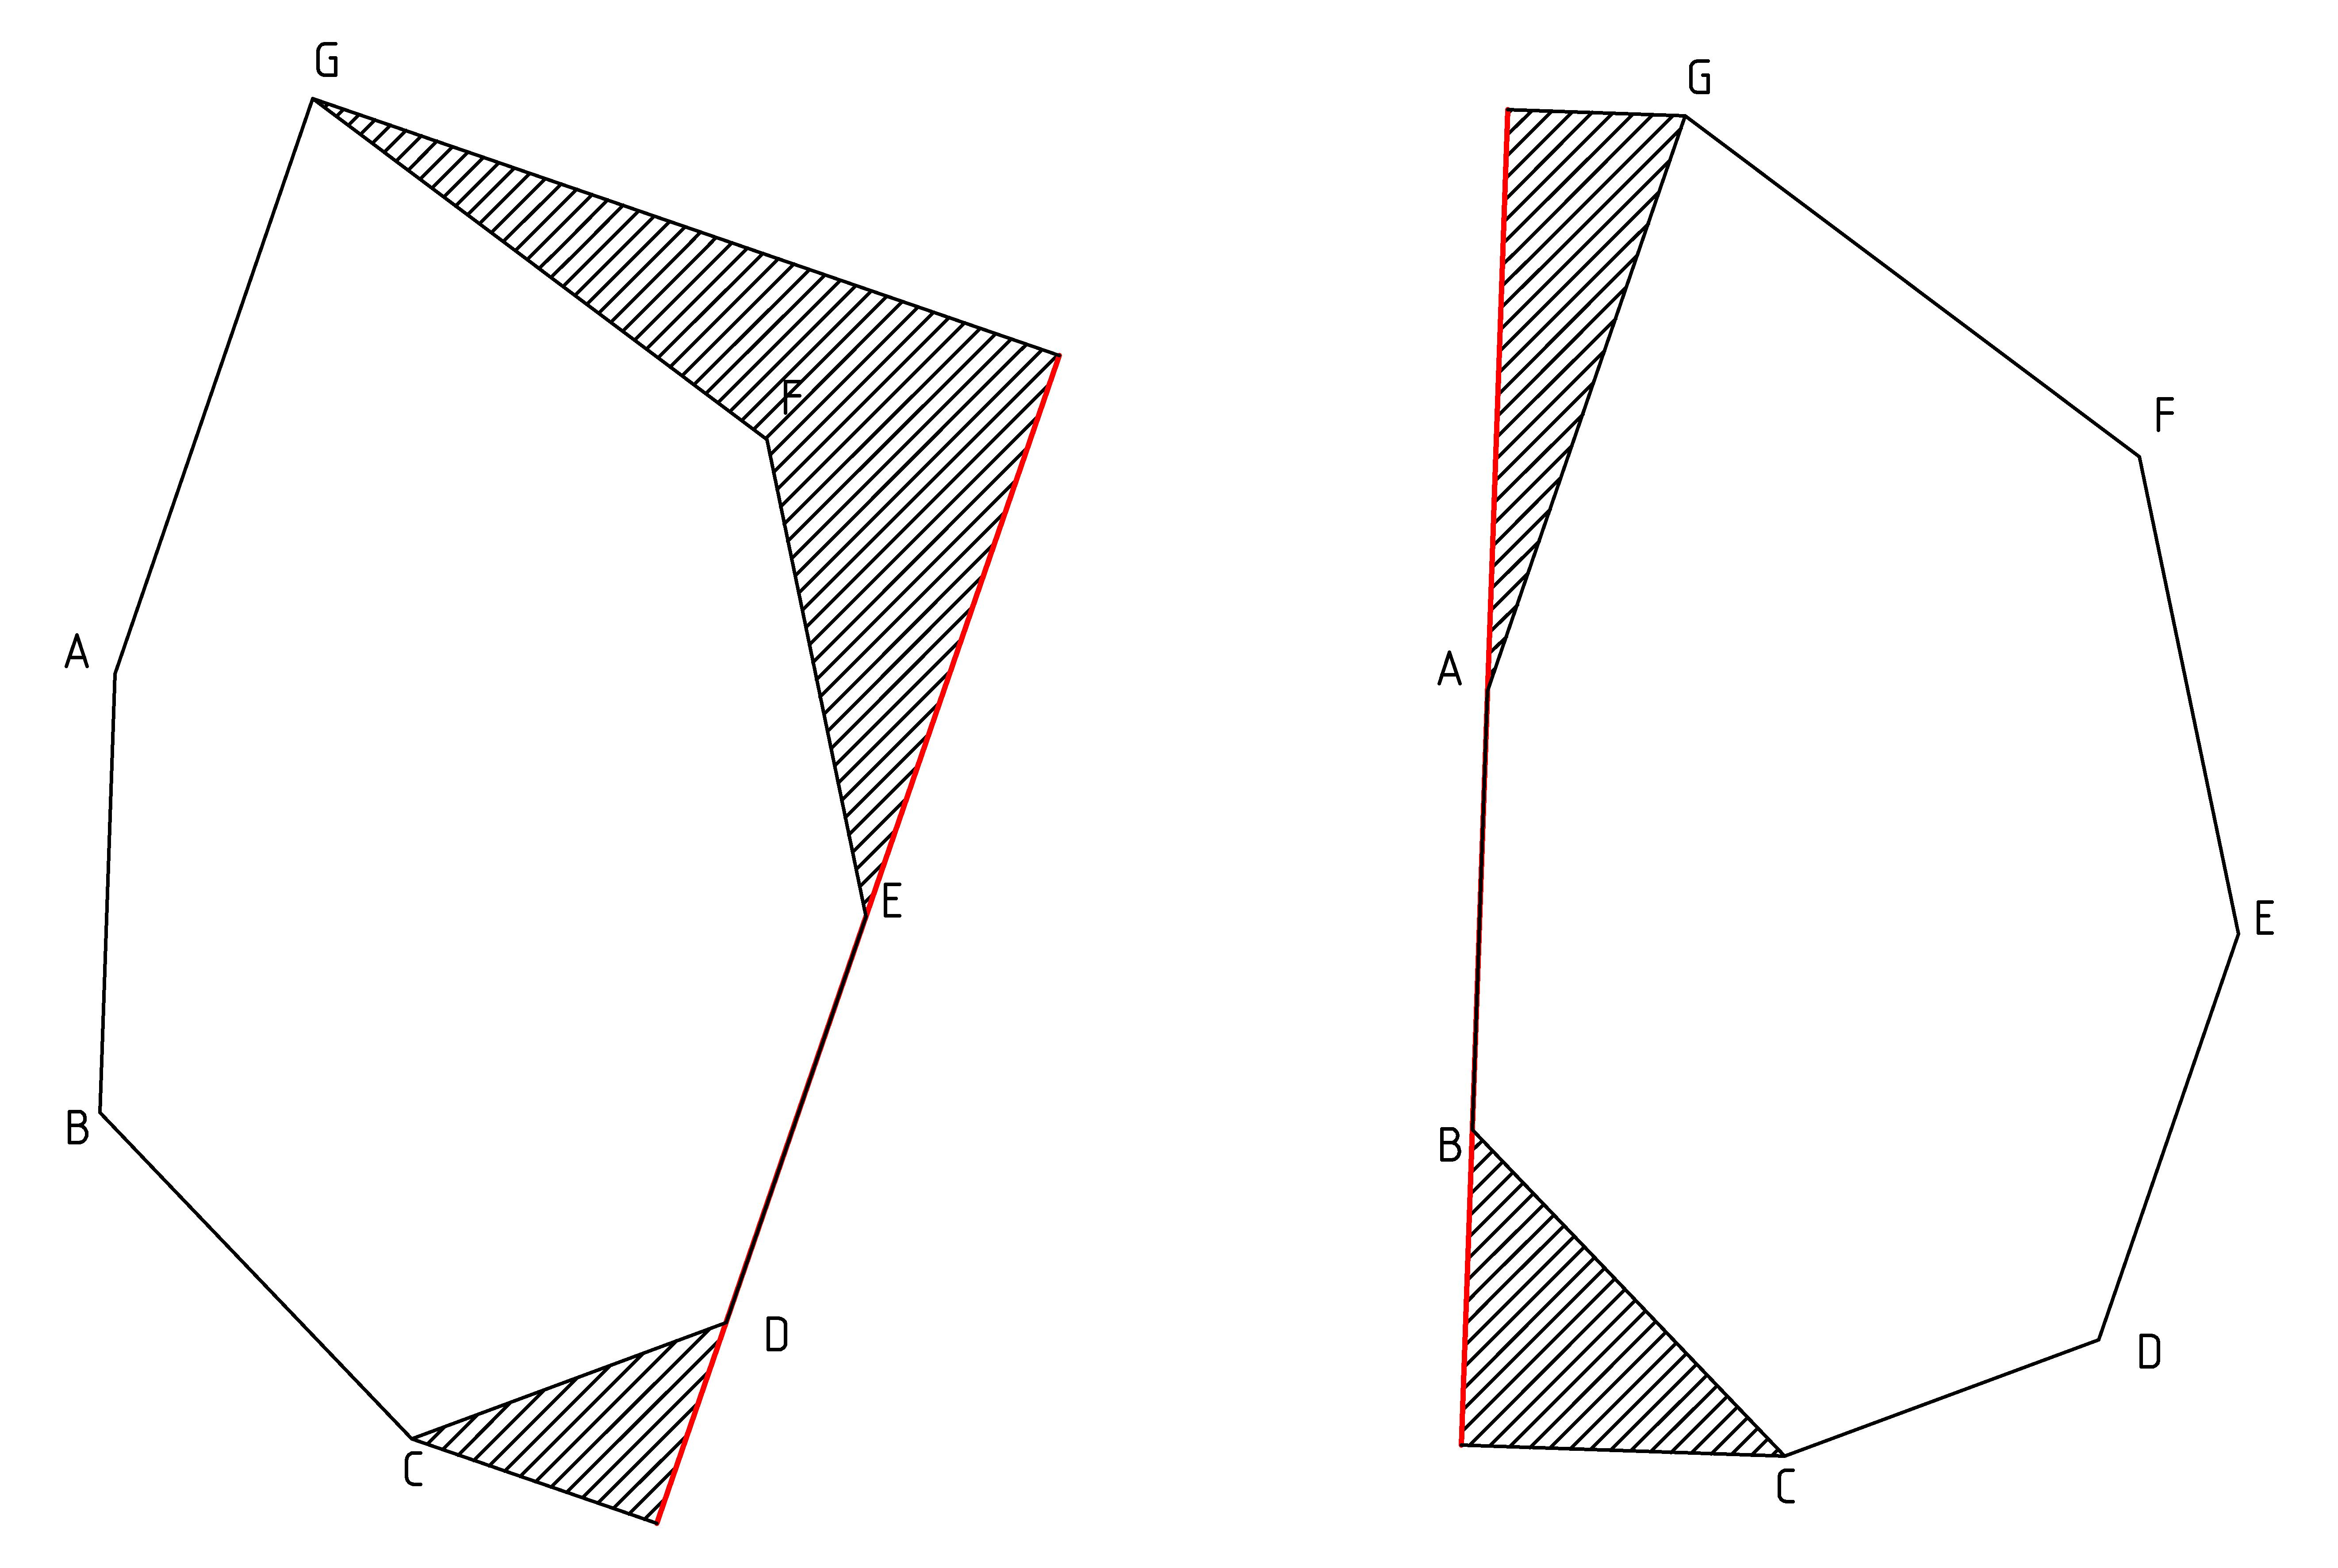
\includegraphics[width=0.8\textwidth]{media/Demo_algorithms/demo_smaller_area.jpg} \\
        \begin{tabular}{l}
            Dimostrazione del criterio di ordinamento degli iperpiani\\
        \end{tabular}
    \end{tabular}
\end{figure}

\begin{center}
    Esempi di approssimazione:
\end{center}
\begin{figure}[H]
    \centering
    \begin{tabular}{ccc}
        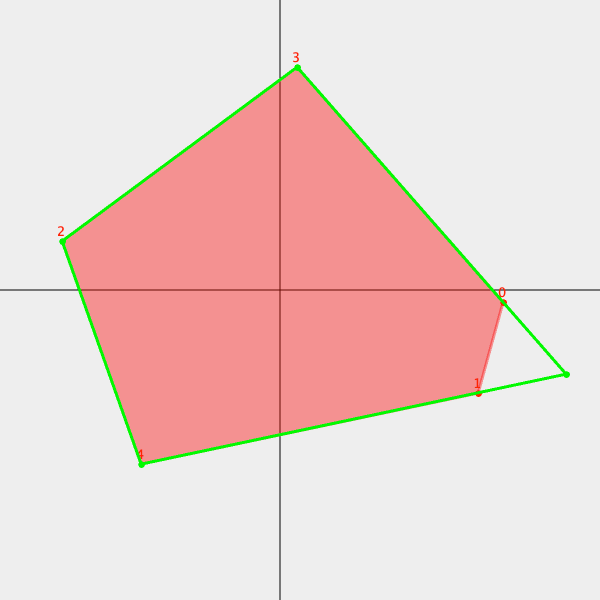
\includegraphics[width=0.3\textwidth]{media/LessArea/5_4.png} &
        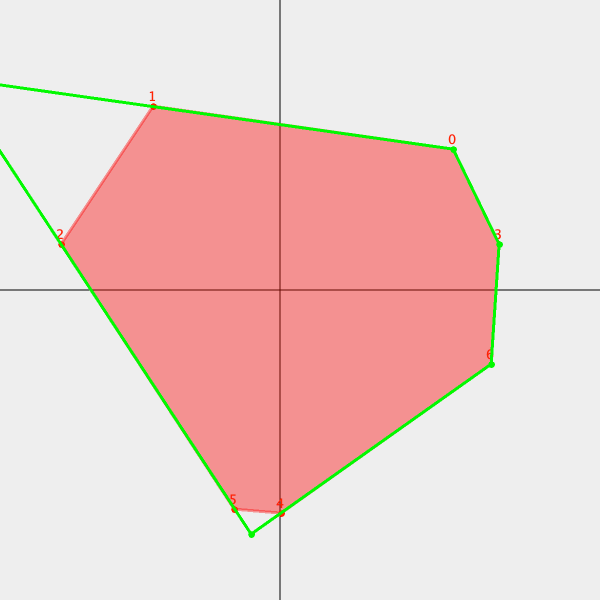
\includegraphics[width=0.3\textwidth]{media/LessArea/7_5.png} &
        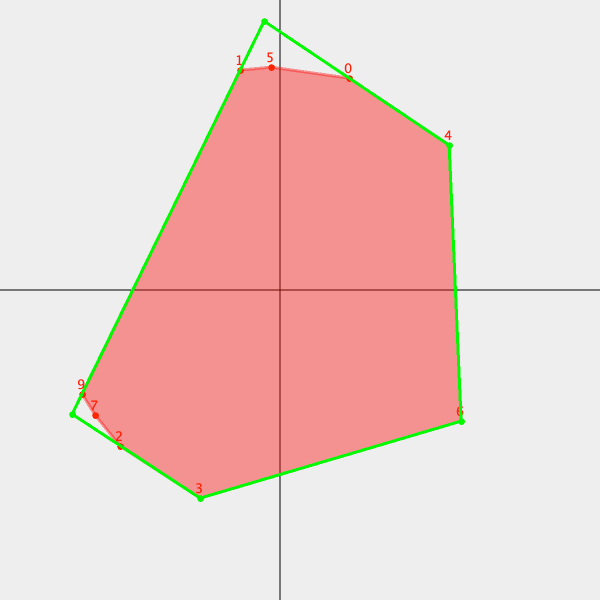
\includegraphics[width=0.3\textwidth]{media/LessArea/9_5.png} \\
        (a) E = 5, h = 4 & (b) E = 7, h = 5 & (c) E = 9, h = 5
    \end{tabular}
\end{figure}

I poligoni prodotti da questo algoritmo tendono a rappresentare in modo accurato 
la forma originale del poligono. 
Tuttavia, l'algoritmo presenta due criticità: la selezione dei lati diventa più 
complessa con l'aumentare del numero di lati del poliedro, poiché in media sarà necessario 
calcolare proiezioni pari alla metà dei lati, e la scelta degli iperpiani non garantisce 
necessariamente la generazione di un politopo chiuso.
 
\pagebreak
\subsection{Ipotesi di Algoritmo Cutting Edges}

Questo algoritmo prevede la graduale selezione degli iperpiani ideali. Questa avviene tramite 
il calcolo delle aree eccedenti per ciascun lato: i lati con le aree eccedenti 
minori saranno scelti per essere approssimati tramite il prolungamento dei lati a loro adiacenti. 

\begin{figure}[H]
    \centering
    \begin{tabular}{c}
        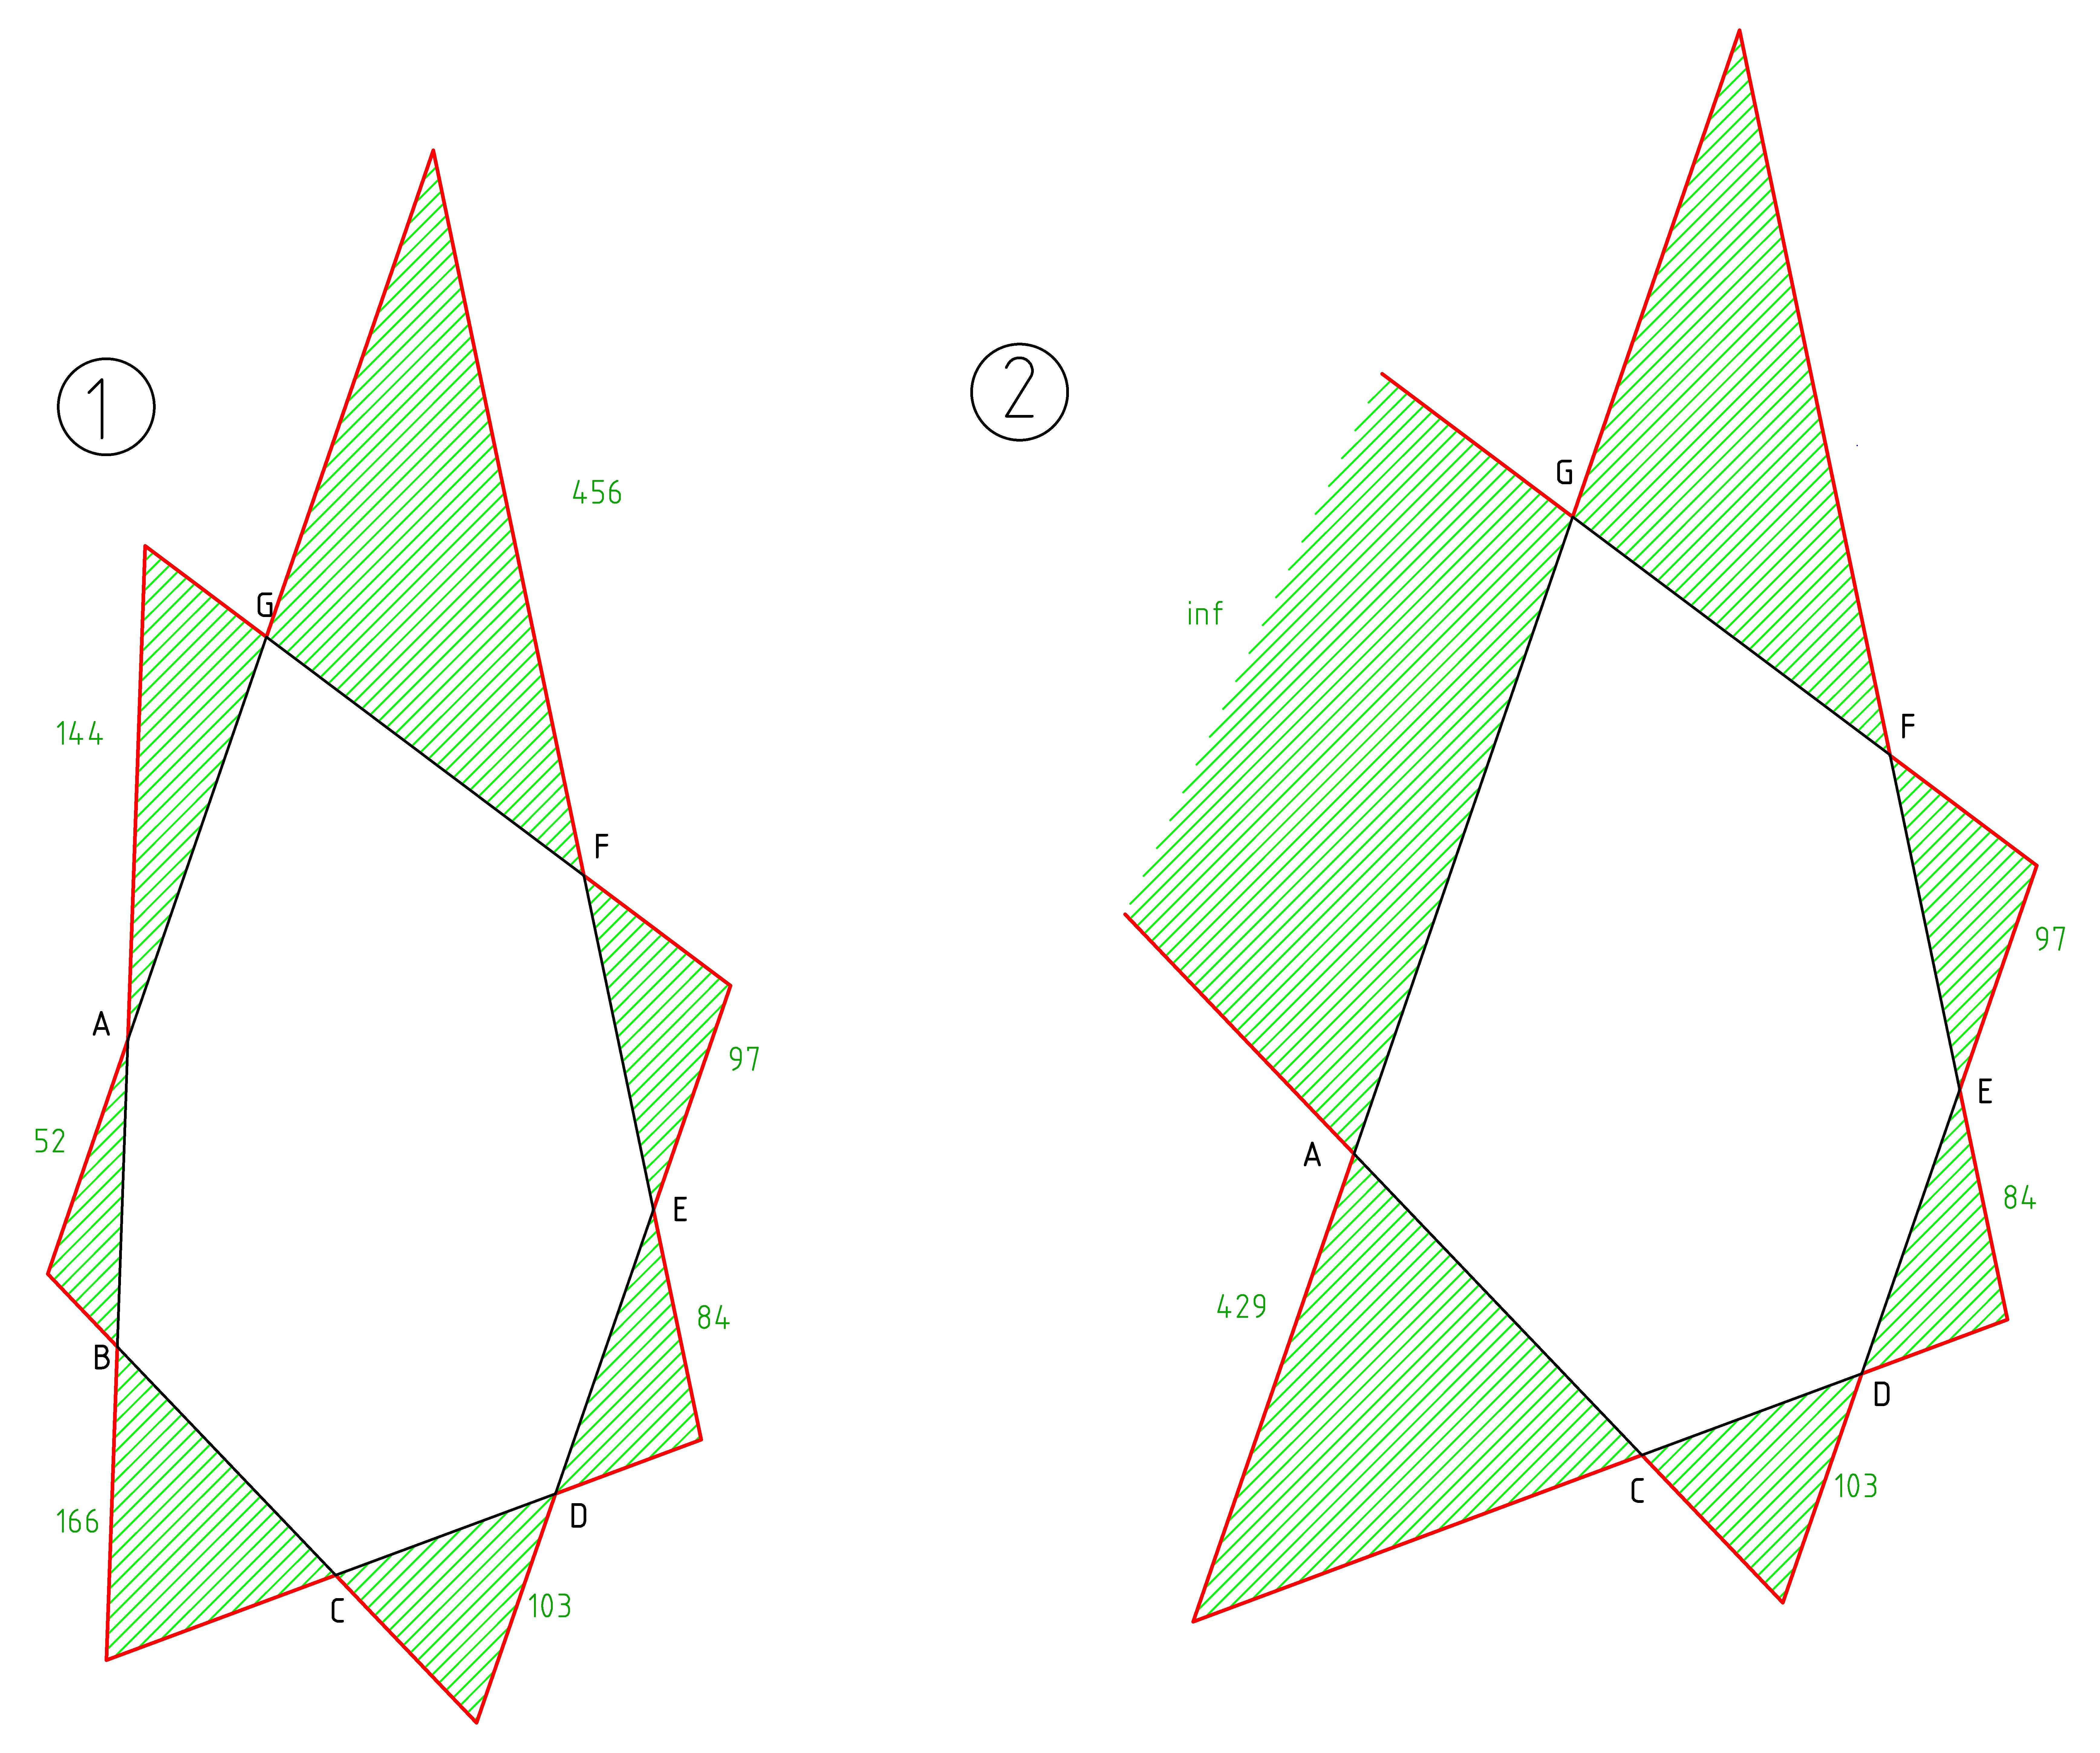
\includegraphics[width=0.8\textwidth]{media/Demo_algorithms/demo_cutting_edges.jpg} \\
        \begin{tabular}{l}
            (1) Dimostrazione del criterio di scelta dell'iperpiano migliore secondo C.E.\\
            (2) Dimostrazione del criterio di scelta sul restante politopo
        \end{tabular}
    \end{tabular}
\end{figure}

\begin{center}
    Esempi di approssimazione:
\end{center}
\begin{figure}[H]
    \centering
    \begin{tabular}{ccc}
        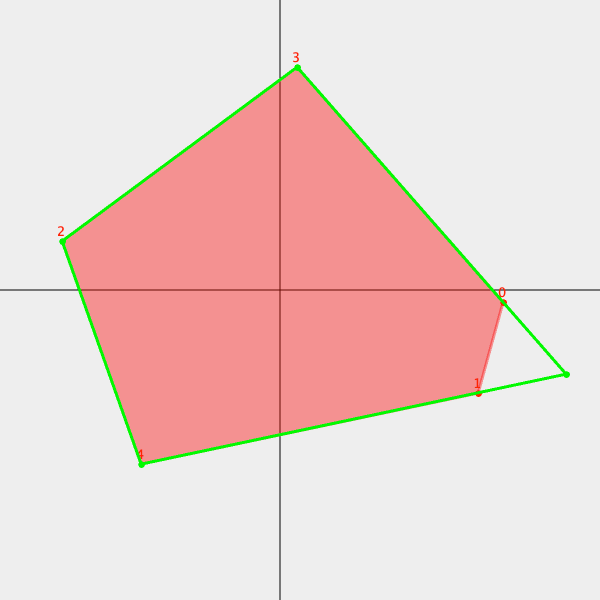
\includegraphics[width=0.3\textwidth]{media/LessArea/5_4.png} &
        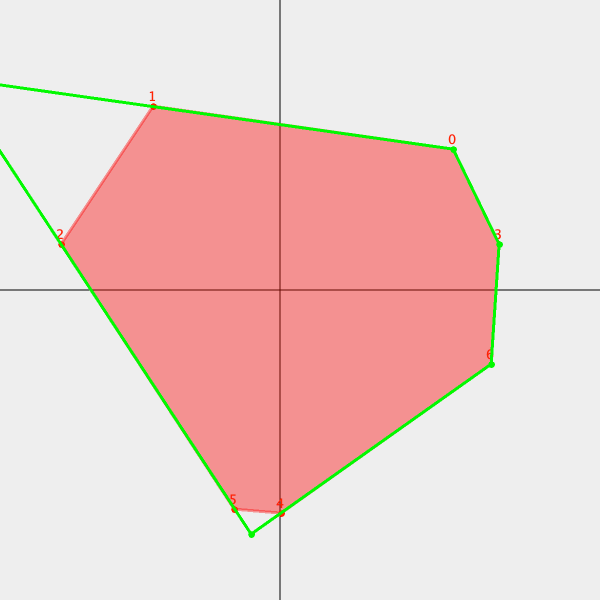
\includegraphics[width=0.3\textwidth]{media/LessArea/7_5.png} &
        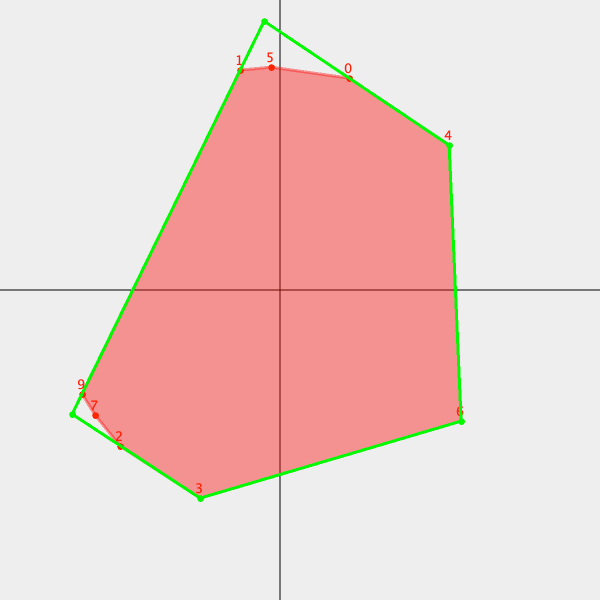
\includegraphics[width=0.3\textwidth]{media/LessArea/9_5.png} \\
        (a) E = 5, h = 4 & (b) E = 7, h = 5 & (c) E = 9, h = 5
    \end{tabular}
\end{figure}

I poligoni generati sembrano rappresentare fedelmente la forma originale del guscio 
convesso e, allo stesso tempo, questi rispettano il vincolo di contenere tutti i punti 
ammissibili del poliedro originale.
L'algoritmo può inoltre trarre vantaggio dall'utilizzo di una mappa per poter 
evitare il ripetuto calcolo delle aree non modificate dall'approssimazione.
\\
